\documentclass{article} % For LaTeX2e
\usepackage{iclr2027_conference,times}

% Optional math commands from https://github.com/goodfeli/dlbook_notation.
%%%%% NEW MATH DEFINITIONS %%%%%

\usepackage{amsmath,amsfonts,bm}

% Mark sections of captions for referring to divisions of figures
\newcommand{\figleft}{{\em (Left)}}
\newcommand{\figcenter}{{\em (Center)}}
\newcommand{\figright}{{\em (Right)}}
\newcommand{\figtop}{{\em (Top)}}
\newcommand{\figbottom}{{\em (Bottom)}}
\newcommand{\captiona}{{\em (a)}}
\newcommand{\captionb}{{\em (b)}}
\newcommand{\captionc}{{\em (c)}}
\newcommand{\captiond}{{\em (d)}}

% Highlight a newly defined term
\newcommand{\newterm}[1]{{\bf #1}}


% Figure reference, lower-case.
\def\figref#1{figure~\ref{#1}}
% Figure reference, capital. For start of sentence
\def\Figref#1{Figure~\ref{#1}}
\def\twofigref#1#2{figures \ref{#1} and \ref{#2}}
\def\quadfigref#1#2#3#4{figures \ref{#1}, \ref{#2}, \ref{#3} and \ref{#4}}
% Section reference, lower-case.
\def\secref#1{section~\ref{#1}}
% Section reference, capital.
\def\Secref#1{Section~\ref{#1}}
% Reference to two sections.
\def\twosecrefs#1#2{sections \ref{#1} and \ref{#2}}
% Reference to three sections.
\def\secrefs#1#2#3{sections \ref{#1}, \ref{#2} and \ref{#3}}
% Reference to an equation, lower-case.
\def\eqref#1{equation~\ref{#1}}
% Reference to an equation, upper case
\def\Eqref#1{Equation~\ref{#1}}
% A raw reference to an equation---avoid using if possible
\def\plaineqref#1{\ref{#1}}
% Reference to a chapter, lower-case.
\def\chapref#1{chapter~\ref{#1}}
% Reference to an equation, upper case.
\def\Chapref#1{Chapter~\ref{#1}}
% Reference to a range of chapters
\def\rangechapref#1#2{chapters\ref{#1}--\ref{#2}}
% Reference to an algorithm, lower-case.
\def\algref#1{algorithm~\ref{#1}}
% Reference to an algorithm, upper case.
\def\Algref#1{Algorithm~\ref{#1}}
\def\twoalgref#1#2{algorithms \ref{#1} and \ref{#2}}
\def\Twoalgref#1#2{Algorithms \ref{#1} and \ref{#2}}
% Reference to a part, lower case
\def\partref#1{part~\ref{#1}}
% Reference to a part, upper case
\def\Partref#1{Part~\ref{#1}}
\def\twopartref#1#2{parts \ref{#1} and \ref{#2}}

\def\ceil#1{\lceil #1 \rceil}
\def\floor#1{\lfloor #1 \rfloor}
\def\1{\bm{1}}
\newcommand{\train}{\mathcal{D}}
\newcommand{\valid}{\mathcal{D_{\mathrm{valid}}}}
\newcommand{\test}{\mathcal{D_{\mathrm{test}}}}

\def\eps{{\epsilon}}


% Random variables
\def\reta{{\textnormal{$\eta$}}}
\def\ra{{\textnormal{a}}}
\def\rb{{\textnormal{b}}}
\def\rc{{\textnormal{c}}}
\def\rd{{\textnormal{d}}}
\def\re{{\textnormal{e}}}
\def\rf{{\textnormal{f}}}
\def\rg{{\textnormal{g}}}
\def\rh{{\textnormal{h}}}
\def\ri{{\textnormal{i}}}
\def\rj{{\textnormal{j}}}
\def\rk{{\textnormal{k}}}
\def\rl{{\textnormal{l}}}
% rm is already a command, just don't name any random variables m
\def\rn{{\textnormal{n}}}
\def\ro{{\textnormal{o}}}
\def\rp{{\textnormal{p}}}
\def\rq{{\textnormal{q}}}
\def\rr{{\textnormal{r}}}
\def\rs{{\textnormal{s}}}
\def\rt{{\textnormal{t}}}
\def\ru{{\textnormal{u}}}
\def\rv{{\textnormal{v}}}
\def\rw{{\textnormal{w}}}
\def\rx{{\textnormal{x}}}
\def\ry{{\textnormal{y}}}
\def\rz{{\textnormal{z}}}

% Random vectors
\def\rvepsilon{{\mathbf{\epsilon}}}
\def\rvtheta{{\mathbf{\theta}}}
\def\rva{{\mathbf{a}}}
\def\rvb{{\mathbf{b}}}
\def\rvc{{\mathbf{c}}}
\def\rvd{{\mathbf{d}}}
\def\rve{{\mathbf{e}}}
\def\rvf{{\mathbf{f}}}
\def\rvg{{\mathbf{g}}}
\def\rvh{{\mathbf{h}}}
\def\rvu{{\mathbf{i}}}
\def\rvj{{\mathbf{j}}}
\def\rvk{{\mathbf{k}}}
\def\rvl{{\mathbf{l}}}
\def\rvm{{\mathbf{m}}}
\def\rvn{{\mathbf{n}}}
\def\rvo{{\mathbf{o}}}
\def\rvp{{\mathbf{p}}}
\def\rvq{{\mathbf{q}}}
\def\rvr{{\mathbf{r}}}
\def\rvs{{\mathbf{s}}}
\def\rvt{{\mathbf{t}}}
\def\rvu{{\mathbf{u}}}
\def\rvv{{\mathbf{v}}}
\def\rvw{{\mathbf{w}}}
\def\rvx{{\mathbf{x}}}
\def\rvy{{\mathbf{y}}}
\def\rvz{{\mathbf{z}}}

% Elements of random vectors
\def\erva{{\textnormal{a}}}
\def\ervb{{\textnormal{b}}}
\def\ervc{{\textnormal{c}}}
\def\ervd{{\textnormal{d}}}
\def\erve{{\textnormal{e}}}
\def\ervf{{\textnormal{f}}}
\def\ervg{{\textnormal{g}}}
\def\ervh{{\textnormal{h}}}
\def\ervi{{\textnormal{i}}}
\def\ervj{{\textnormal{j}}}
\def\ervk{{\textnormal{k}}}
\def\ervl{{\textnormal{l}}}
\def\ervm{{\textnormal{m}}}
\def\ervn{{\textnormal{n}}}
\def\ervo{{\textnormal{o}}}
\def\ervp{{\textnormal{p}}}
\def\ervq{{\textnormal{q}}}
\def\ervr{{\textnormal{r}}}
\def\ervs{{\textnormal{s}}}
\def\ervt{{\textnormal{t}}}
\def\ervu{{\textnormal{u}}}
\def\ervv{{\textnormal{v}}}
\def\ervw{{\textnormal{w}}}
\def\ervx{{\textnormal{x}}}
\def\ervy{{\textnormal{y}}}
\def\ervz{{\textnormal{z}}}

% Random matrices
\def\rmA{{\mathbf{A}}}
\def\rmB{{\mathbf{B}}}
\def\rmC{{\mathbf{C}}}
\def\rmD{{\mathbf{D}}}
\def\rmE{{\mathbf{E}}}
\def\rmF{{\mathbf{F}}}
\def\rmG{{\mathbf{G}}}
\def\rmH{{\mathbf{H}}}
\def\rmI{{\mathbf{I}}}
\def\rmJ{{\mathbf{J}}}
\def\rmK{{\mathbf{K}}}
\def\rmL{{\mathbf{L}}}
\def\rmM{{\mathbf{M}}}
\def\rmN{{\mathbf{N}}}
\def\rmO{{\mathbf{O}}}
\def\rmP{{\mathbf{P}}}
\def\rmQ{{\mathbf{Q}}}
\def\rmR{{\mathbf{R}}}
\def\rmS{{\mathbf{S}}}
\def\rmT{{\mathbf{T}}}
\def\rmU{{\mathbf{U}}}
\def\rmV{{\mathbf{V}}}
\def\rmW{{\mathbf{W}}}
\def\rmX{{\mathbf{X}}}
\def\rmY{{\mathbf{Y}}}
\def\rmZ{{\mathbf{Z}}}

% Elements of random matrices
\def\ermA{{\textnormal{A}}}
\def\ermB{{\textnormal{B}}}
\def\ermC{{\textnormal{C}}}
\def\ermD{{\textnormal{D}}}
\def\ermE{{\textnormal{E}}}
\def\ermF{{\textnormal{F}}}
\def\ermG{{\textnormal{G}}}
\def\ermH{{\textnormal{H}}}
\def\ermI{{\textnormal{I}}}
\def\ermJ{{\textnormal{J}}}
\def\ermK{{\textnormal{K}}}
\def\ermL{{\textnormal{L}}}
\def\ermM{{\textnormal{M}}}
\def\ermN{{\textnormal{N}}}
\def\ermO{{\textnormal{O}}}
\def\ermP{{\textnormal{P}}}
\def\ermQ{{\textnormal{Q}}}
\def\ermR{{\textnormal{R}}}
\def\ermS{{\textnormal{S}}}
\def\ermT{{\textnormal{T}}}
\def\ermU{{\textnormal{U}}}
\def\ermV{{\textnormal{V}}}
\def\ermW{{\textnormal{W}}}
\def\ermX{{\textnormal{X}}}
\def\ermY{{\textnormal{Y}}}
\def\ermZ{{\textnormal{Z}}}

% Vectors
\def\vzero{{\bm{0}}}
\def\vone{{\bm{1}}}
\def\vmu{{\bm{\mu}}}
\def\vtheta{{\bm{\theta}}}
\def\va{{\bm{a}}}
\def\vb{{\bm{b}}}
\def\vc{{\bm{c}}}
\def\vd{{\bm{d}}}
\def\ve{{\bm{e}}}
\def\vf{{\bm{f}}}
\def\vg{{\bm{g}}}
\def\vh{{\bm{h}}}
\def\vi{{\bm{i}}}
\def\vj{{\bm{j}}}
\def\vk{{\bm{k}}}
\def\vl{{\bm{l}}}
\def\vm{{\bm{m}}}
\def\vn{{\bm{n}}}
\def\vo{{\bm{o}}}
\def\vp{{\bm{p}}}
\def\vq{{\bm{q}}}
\def\vr{{\bm{r}}}
\def\vs{{\bm{s}}}
\def\vt{{\bm{t}}}
\def\vu{{\bm{u}}}
\def\vv{{\bm{v}}}
\def\vw{{\bm{w}}}
\def\vx{{\bm{x}}}
\def\vy{{\bm{y}}}
\def\vz{{\bm{z}}}

% Elements of vectors
\def\evalpha{{\alpha}}
\def\evbeta{{\beta}}
\def\evepsilon{{\epsilon}}
\def\evlambda{{\lambda}}
\def\evomega{{\omega}}
\def\evmu{{\mu}}
\def\evpsi{{\psi}}
\def\evsigma{{\sigma}}
\def\evtheta{{\theta}}
\def\eva{{a}}
\def\evb{{b}}
\def\evc{{c}}
\def\evd{{d}}
\def\eve{{e}}
\def\evf{{f}}
\def\evg{{g}}
\def\evh{{h}}
\def\evi{{i}}
\def\evj{{j}}
\def\evk{{k}}
\def\evl{{l}}
\def\evm{{m}}
\def\evn{{n}}
\def\evo{{o}}
\def\evp{{p}}
\def\evq{{q}}
\def\evr{{r}}
\def\evs{{s}}
\def\evt{{t}}
\def\evu{{u}}
\def\evv{{v}}
\def\evw{{w}}
\def\evx{{x}}
\def\evy{{y}}
\def\evz{{z}}

% Matrix
\def\mA{{\bm{A}}}
\def\mB{{\bm{B}}}
\def\mC{{\bm{C}}}
\def\mD{{\bm{D}}}
\def\mE{{\bm{E}}}
\def\mF{{\bm{F}}}
\def\mG{{\bm{G}}}
\def\mH{{\bm{H}}}
\def\mI{{\bm{I}}}
\def\mJ{{\bm{J}}}
\def\mK{{\bm{K}}}
\def\mL{{\bm{L}}}
\def\mM{{\bm{M}}}
\def\mN{{\bm{N}}}
\def\mO{{\bm{O}}}
\def\mP{{\bm{P}}}
\def\mQ{{\bm{Q}}}
\def\mR{{\bm{R}}}
\def\mS{{\bm{S}}}
\def\mT{{\bm{T}}}
\def\mU{{\bm{U}}}
\def\mV{{\bm{V}}}
\def\mW{{\bm{W}}}
\def\mX{{\bm{X}}}
\def\mY{{\bm{Y}}}
\def\mZ{{\bm{Z}}}
\def\mBeta{{\bm{\beta}}}
\def\mPhi{{\bm{\Phi}}}
\def\mLambda{{\bm{\Lambda}}}
\def\mSigma{{\bm{\Sigma}}}

% Tensor
\DeclareMathAlphabet{\mathsfit}{\encodingdefault}{\sfdefault}{m}{sl}
\SetMathAlphabet{\mathsfit}{bold}{\encodingdefault}{\sfdefault}{bx}{n}
\newcommand{\tens}[1]{\bm{\mathsfit{#1}}}
\def\tA{{\tens{A}}}
\def\tB{{\tens{B}}}
\def\tC{{\tens{C}}}
\def\tD{{\tens{D}}}
\def\tE{{\tens{E}}}
\def\tF{{\tens{F}}}
\def\tG{{\tens{G}}}
\def\tH{{\tens{H}}}
\def\tI{{\tens{I}}}
\def\tJ{{\tens{J}}}
\def\tK{{\tens{K}}}
\def\tL{{\tens{L}}}
\def\tM{{\tens{M}}}
\def\tN{{\tens{N}}}
\def\tO{{\tens{O}}}
\def\tP{{\tens{P}}}
\def\tQ{{\tens{Q}}}
\def\tR{{\tens{R}}}
\def\tS{{\tens{S}}}
\def\tT{{\tens{T}}}
\def\tU{{\tens{U}}}
\def\tV{{\tens{V}}}
\def\tW{{\tens{W}}}
\def\tX{{\tens{X}}}
\def\tY{{\tens{Y}}}
\def\tZ{{\tens{Z}}}


% Graph
\def\gA{{\mathcal{A}}}
\def\gB{{\mathcal{B}}}
\def\gC{{\mathcal{C}}}
\def\gD{{\mathcal{D}}}
\def\gE{{\mathcal{E}}}
\def\gF{{\mathcal{F}}}
\def\gG{{\mathcal{G}}}
\def\gH{{\mathcal{H}}}
\def\gI{{\mathcal{I}}}
\def\gJ{{\mathcal{J}}}
\def\gK{{\mathcal{K}}}
\def\gL{{\mathcal{L}}}
\def\gM{{\mathcal{M}}}
\def\gN{{\mathcal{N}}}
\def\gO{{\mathcal{O}}}
\def\gP{{\mathcal{P}}}
\def\gQ{{\mathcal{Q}}}
\def\gR{{\mathcal{R}}}
\def\gS{{\mathcal{S}}}
\def\gT{{\mathcal{T}}}
\def\gU{{\mathcal{U}}}
\def\gV{{\mathcal{V}}}
\def\gW{{\mathcal{W}}}
\def\gX{{\mathcal{X}}}
\def\gY{{\mathcal{Y}}}
\def\gZ{{\mathcal{Z}}}

% Sets
\def\sA{{\mathbb{A}}}
\def\sB{{\mathbb{B}}}
\def\sC{{\mathbb{C}}}
\def\sD{{\mathbb{D}}}
% Don't use a set called E, because this would be the same as our symbol
% for expectation.
\def\sF{{\mathbb{F}}}
\def\sG{{\mathbb{G}}}
\def\sH{{\mathbb{H}}}
\def\sI{{\mathbb{I}}}
\def\sJ{{\mathbb{J}}}
\def\sK{{\mathbb{K}}}
\def\sL{{\mathbb{L}}}
\def\sM{{\mathbb{M}}}
\def\sN{{\mathbb{N}}}
\def\sO{{\mathbb{O}}}
\def\sP{{\mathbb{P}}}
\def\sQ{{\mathbb{Q}}}
\def\sR{{\mathbb{R}}}
\def\sS{{\mathbb{S}}}
\def\sT{{\mathbb{T}}}
\def\sU{{\mathbb{U}}}
\def\sV{{\mathbb{V}}}
\def\sW{{\mathbb{W}}}
\def\sX{{\mathbb{X}}}
\def\sY{{\mathbb{Y}}}
\def\sZ{{\mathbb{Z}}}

% Entries of a matrix
\def\emLambda{{\Lambda}}
\def\emA{{A}}
\def\emB{{B}}
\def\emC{{C}}
\def\emD{{D}}
\def\emE{{E}}
\def\emF{{F}}
\def\emG{{G}}
\def\emH{{H}}
\def\emI{{I}}
\def\emJ{{J}}
\def\emK{{K}}
\def\emL{{L}}
\def\emM{{M}}
\def\emN{{N}}
\def\emO{{O}}
\def\emP{{P}}
\def\emQ{{Q}}
\def\emR{{R}}
\def\emS{{S}}
\def\emT{{T}}
\def\emU{{U}}
\def\emV{{V}}
\def\emW{{W}}
\def\emX{{X}}
\def\emY{{Y}}
\def\emZ{{Z}}
\def\emSigma{{\Sigma}}

% entries of a tensor
% Same font as tensor, without \bm wrapper
\newcommand{\etens}[1]{\mathsfit{#1}}
\def\etLambda{{\etens{\Lambda}}}
\def\etA{{\etens{A}}}
\def\etB{{\etens{B}}}
\def\etC{{\etens{C}}}
\def\etD{{\etens{D}}}
\def\etE{{\etens{E}}}
\def\etF{{\etens{F}}}
\def\etG{{\etens{G}}}
\def\etH{{\etens{H}}}
\def\etI{{\etens{I}}}
\def\etJ{{\etens{J}}}
\def\etK{{\etens{K}}}
\def\etL{{\etens{L}}}
\def\etM{{\etens{M}}}
\def\etN{{\etens{N}}}
\def\etO{{\etens{O}}}
\def\etP{{\etens{P}}}
\def\etQ{{\etens{Q}}}
\def\etR{{\etens{R}}}
\def\etS{{\etens{S}}}
\def\etT{{\etens{T}}}
\def\etU{{\etens{U}}}
\def\etV{{\etens{V}}}
\def\etW{{\etens{W}}}
\def\etX{{\etens{X}}}
\def\etY{{\etens{Y}}}
\def\etZ{{\etens{Z}}}

% The true underlying data generating distribution
\newcommand{\pdata}{p_{\rm{data}}}
% The empirical distribution defined by the training set
\newcommand{\ptrain}{\hat{p}_{\rm{data}}}
\newcommand{\Ptrain}{\hat{P}_{\rm{data}}}
% The model distribution
\newcommand{\pmodel}{p_{\rm{model}}}
\newcommand{\Pmodel}{P_{\rm{model}}}
\newcommand{\ptildemodel}{\tilde{p}_{\rm{model}}}
% Stochastic autoencoder distributions
\newcommand{\pencode}{p_{\rm{encoder}}}
\newcommand{\pdecode}{p_{\rm{decoder}}}
\newcommand{\precons}{p_{\rm{reconstruct}}}

\newcommand{\laplace}{\mathrm{Laplace}} % Laplace distribution

\newcommand{\E}{\mathbb{E}}
\newcommand{\Ls}{\mathcal{L}}
\newcommand{\R}{\mathbb{R}}
\newcommand{\emp}{\tilde{p}}
\newcommand{\lr}{\alpha}
\newcommand{\reg}{\lambda}
\newcommand{\rect}{\mathrm{rectifier}}
\newcommand{\softmax}{\mathrm{softmax}}
\newcommand{\sigmoid}{\sigma}
\newcommand{\softplus}{\zeta}
\newcommand{\KL}{D_{\mathrm{KL}}}
\newcommand{\Var}{\mathrm{Var}}
\newcommand{\standarderror}{\mathrm{SE}}
\newcommand{\Cov}{\mathrm{Cov}}
% Wolfram Mathworld says $L^2$ is for function spaces and $\ell^2$ is for vectors
% But then they seem to use $L^2$ for vectors throughout the site, and so does
% wikipedia.
\newcommand{\normlzero}{L^0}
\newcommand{\normlone}{L^1}
\newcommand{\normltwo}{L^2}
\newcommand{\normlp}{L^p}
\newcommand{\normmax}{L^\infty}

\newcommand{\parents}{Pa} % See usage in notation.tex. Chosen to match Daphne's book.

\DeclareMathOperator*{\argmax}{arg\,max}
\DeclareMathOperator*{\argmin}{arg\,min}

\DeclareMathOperator{\sign}{sign}
\DeclareMathOperator{\Tr}{Tr}
\let\ab\allowbreak


\usepackage{hyperref}
\usepackage{url}
\usepackage{booktabs}
\usepackage{multirow}
\usepackage{graphicx}

% The ICLR style sets \flushbottom, which forces every page to the full text
% height; on pages that cannot be filled the slack is stretched into
% \textfloatsep, leaving a large gap under each table. Let pages run short
% instead.
\raggedbottom

% Tighten the default float separations (\textfloatsep is 20pt in article).
\setlength{\textfloatsep}{2pt plus 1pt minus 1pt}
\setlength{\floatsep}{2pt plus 1pt minus 1pt}
\setlength{\intextsep}{2pt plus 1pt minus 1pt}
\setlength{\abovecaptionskip}{4pt}
\setlength{\belowcaptionskip}{2pt}

\title{EGRD: Assessing Research Novelty through\\
Evidence-Grounded Residual Decomposition}

% Authors must not appear in the submitted version.
\author{Anonymous Authors}

%\iclrfinalcopy % Uncomment for camera-ready version, but NOT for submission.
\begin{document}

\maketitle

\begin{abstract}
Assessing the novelty of a research idea requires identifying what remains
beyond prior work, even when coverage is dispersed across several papers or
the contribution lies in a new combination of familiar components. We propose
Evidence-Grounded Residual Decomposition (EGRD), a supervised framework for
predicting ordered novelty grades relative to an explicit set of prior works
published before the target. EGRD decomposes the target into latent semantic
units and learns a support matrix aligning each unit with each prior.
Aggregating support across priors yields unit residuals for insufficiently
covered content, while within-prior co-support yields interaction residuals
for potentially novel combinations. The model predicts novelty from these
residuals together with coverage and contextual representations. To support
training and evaluation, we construct \textsc{IdeaDelta}, which pairs research
ideas with temporally admissible priors and provides model-generated coverage
and novelty annotations across graph machine learning, computer vision, and
time series. On temporally held-out ideas, EGRD consistently outperforms
prompted baselines across these domains, whether those baselines read the same
evidence or select their own priors from the same admissible pool.
In a separate transfer experiment, the frozen model evaluated against the
expert labels of RINoBench yields higher ordinal agreement and Macro-F1 than
the systems that benchmark reports. Ablations show that predictions depend on
matched prior evidence and benefit from aggregating support across priors and
representing residual contributions.
\end{abstract}

\section{Introduction}
\label{sec:intro}

Judging whether a research idea is new is difficult, and the growing volume of
published work makes it harder. Novelty is not a monotone function of textual
similarity to any single prior work, and separating a genuine advance from a
restatement is in practice a judgment that draws on familiarity with the field.
We therefore study \emph{evidence-conditioned} novelty assessment: grading a
target idea relative to an explicit set of prior works published before it.
Fixing this set makes the basis of each judgment inspectable and turns the
evidence into a variable that can be controlled.

Much existing work takes a paper as the unit of assessment, from citation-pattern
measures \citep{uzzi2013atypical} to document-level embeddings
\citep{cohan2020specter,ostendorff2022scincl} and to systems that review a
submission as a whole \citep{zhu2025deepreview}. A paper bundles contributions of
uneven novelty: a central mechanism may sit beside incidental variants, and one
score over the bundle does not say which contribution it is about. The decision
of what to pursue is made one idea at a time.

Systems that do operate on ideas assemble the judgment as a language-model
workflow, retrieving related work and then prompting a model to compare against
it \citep{wang2024scimon,dasilva2025graphmind,afzal2026beyond}. Both halves are
fragile. The evidence is selected by the system being evaluated, so a verdict
cannot be attributed to the retrieval or to the comparison, and neither can be
measured or improved on its own. The comparison itself is elicited by a prompt
rather than learned against supervision. \citet{schopf2026rinobench} evaluate
this arrangement against expert judgments and report that although the reasoning
such models produce closely mirrors human rationales, that alignment does not
reliably translate into accurate novelty judgments, which diverge significantly
from the expert gold standard.

Such a workflow also compresses the comparison into a single score, and three
distinctions do not survive that compression. Historical coverage can be
\emph{dispersed}: several papers may jointly account for an idea even when no
single paper closely resembles it, so a comparison against the nearest prior
work misses it. Ideas at equal coverage differ in \emph{what remains}: one may
leave only an implementation detail unexplained while another introduces a new
mechanism. And components that are individually covered may form a
\emph{combination} that no single prior work puts together. Each is a question
about a particular part of the idea and the particular prior work responsible
for it, and a score that discards this correspondence cannot be post-processed
to recover it. Assessing novelty calls instead for a representation that keeps
it: which prior work accounts for which part of the target, and what is left
over.

Studying this setting requires ideas paired with the evidence admissible at the
time they were proposed, which existing novelty benchmarks do not provide. We
therefore construct \textsc{IdeaDelta}, a dataset spanning graph machine
learning, computer vision, and time series, in which every entry is an
idea-length statement paired with
temporally admissible priors and annotated at both the idea and target--prior
levels. The pairing supports the proposed task and makes controlled changes to
the supplied evidence possible.

We propose Evidence-Grounded Residual Decomposition (EGRD), which decomposes a
target against ranked historical evidence into what that evidence accounts for
and what it leaves, and predicts an ordered novelty grade from the two. For
larger evidence sets, a conservative blockwise inference rule extends the
evidence budget without retraining. Our contributions are:
\begin{itemize}
  \item \textbf{\textsc{IdeaDelta}, a multi-domain, evidence-paired dataset.}
  We provide ideas paired
  with temporally admissible priors and annotations of coverage, residual
  contribution, and novelty across three research areas. Because the evidence is
  supplied rather than retrieved, it can be intervened on: permuting the priors
  while holding the target fixed drops the model to near-chance in every domain.
  \item \textbf{Unit-level coverage over dispersed evidence.} We model how much
  of the target the supplied priors account for at the level of latent semantic
  units rather than of the idea as a whole. A learned support matrix aligns each
  unit with each prior, and noisy-OR aggregation lets several partially relevant
  papers jointly cover a unit that none of them covers alone.
  \item \textbf{Typed residuals.} We represent what the priors leave unaccounted
  for as two distinct quantities: unit residuals, for content that no prior
  supports, and interaction residuals, for combinations of individually covered
  components that no single prior puts together. Both are read off the same
  support matrix, so the distinction between an unexplored contribution and an
  effective recombination is produced by the model rather than asserted.
\end{itemize}

Appendix~\ref{app:related} situates EGRD against automated idea generation,
prior novelty judges, and decomposed verification against evidence.


% \input{sections/problem}
% Dataset section. Main text is deliberately short: design and composition
% here, procedure and validity evidence in Appendix A (sections/dataset_details).
%
% Dataset: dataset/multi_domain_dataset/. Every number below was read from the
% data files themselves, not from any summary document:
%   */dataset_manifest.json              counts, label distributions, date range
%   mixed/idea_novelty_dataset.jsonl     per-domain novelty distribution (the
%       dataset carries a native `domain` field; nothing is recovered by matching)
%   mixed/pair_staged/*.jsonl            pair split sizes
% Idea-level split sizes follow from applying the pair_staged date cuts
% (< 202502, 202502--202510, >= 202511) to target_date; they are reproducible
% from idea_novelty_dataset.jsonl alone.
%
% OPEN: Section 5 and Section 6 still carry numbers from the earlier 25,435-row
% build (3,816 test / 3,177 domain-identified / 17,804-3,815-3,816 splits) and
% need replacing with results measured on this dataset.

\section{Dataset}
\label{sec:dataset}

Novelty can only be assessed relative to earlier work. Each evaluation example
must therefore specify a target idea, the prior ideas available when it was
proposed, and the contribution that remains after accounting for those priors.
We construct \textsc{IdeaDelta} to provide these three elements.

\subsection{Task and labels}
\label{sec:dataset-task}

The unit of annotation is a research \emph{idea}: one innovation claim extracted
from a paper. For example, a paper that introduces both a new objective and a
new architecture contributes two ideas, which are evaluated separately. Let
$x$ denote a target idea published at time $t_x$. Its admissible priors are
$\mathcal{P}_x=\{p_k\mid t_{p_k}<t_x\}$. This temporal constraint is essential:
an idea published after the target cannot serve as evidence about the target's
novelty, regardless of its semantic similarity. We annotate each target--prior
pair with one of four coverage levels and each target with an ordered novelty
grade from \textsc{low} to \textsc{high}.

Rather than assign novelty as a single overall impression, we derive it from
four annotated quantities:
\begin{equation}
 \mathrm{raw}(x)=\bigl(1-C_x\bigr)\cdot\Delta_x\cdot E_x\cdot
                 \bigl(1-\lambda S_x\bigr),
 \qquad \lambda=0.45,
 \label{eq:novelty-rule}
\end{equation}
where $C_x$ measures how much of the target is jointly covered by the retained
priors, $\Delta_x$ measures the substantive contribution that remains,
$E_x$ measures whether the retrieved evidence is sufficient for assessment,
and $S_x$ measures how much of the claimed difference is merely surface-level.
We convert the resulting score into the four ordered novelty grades. The rule
assigns lower novelty when prior work already covers the target, when the
remaining difference is not substantive, when the available evidence is
insufficient, or when the difference consists mainly of renaming or other
surface changes.

\subsection{Construction}
\label{sec:dataset-construction}

\paragraph{Paper selection and idea extraction.}
We collect arXiv papers from graph machine learning, computer vision, and time
series. We prioritize papers that were subsequently published, especially at
major venues. An LLM extracts innovation claims from the title, abstract, and
introduction. A second pass removes statements that do not describe a
substantive research contribution, including open-source announcements, bare
state-of-the-art claims, and engineering deliverables.

\paragraph{Prior retrieval.}
For each target, nearest-neighbor search over idea embeddings retrieves
candidate priors published before the target. An LLM adjudicates candidates in
the uncertain similarity range. We also perform a cross-type retrieval pass so
that a target can be linked to relevant prior work of another contribution type.
All target--prior pairs remain within the same research domain.

\paragraph{Annotation.}
The same judge, \texttt{deepseek-v4-pro}, annotates all stages. It first assigns
pairwise coverage labels, with ambiguous cases judged from their technical
content. It then estimates joint coverage, the remaining substantive
contribution, evidence sufficiency, and surface-level difference for each
target. Equation~(\ref{eq:novelty-rule}) converts these quantities into the
idea-level novelty grade. The labels are model-generated, and we manually
inspect samples from each stage. Appendix~\ref{app:dataset} describes the full
pipeline.

\subsection{Composition}
\label{sec:dataset-composition}

\textsc{IdeaDelta} contains $21{,}111$ annotated ideas and $92{,}876$ annotated
target--prior pairs, with target dates ranging from 2019-01 to 2026-09
(Table~\ref{tab:dataset-composition}). Each idea records its source domain, and
the \emph{All} column is the union of the three domain subsets rather than an
additional collection. We order the train, validation, and test splits by date,
with cut points at 2025-02 and 2025-11. The resulting splits contain
$59{,}269/16{,}436/17{,}171$ pairs and $13{,}815/3{,}944/3{,}352$ ideas.

\begin{table}[t]
\centering
\small
\setlength{\tabcolsep}{6pt}
\caption{Dataset composition. Counts of ideas and of target--prior pairs, and the
idea-level novelty distribution. Pairs are formed within a source domain only.}
\label{tab:dataset-composition}
\begin{tabular}{@{}lrrrr@{}}
\toprule
& Graph ML & Computer vision & Time series & All \\
\midrule
Ideas & 5{,}225 & 8{,}291 & 7{,}595 & 21{,}111 \\
Pairs & 21{,}183 & 36{,}238 & 35{,}455 & 92{,}876 \\
\addlinespace
\textsc{low} & 819 & 901 & 1{,}724 & 3{,}444 \\
\textsc{weak} & 1{,}240 & 1{,}711 & 1{,}614 & 4{,}565 \\
\textsc{moderate} & 2{,}247 & 2{,}777 & 2{,}173 & 7{,}197 \\
\textsc{high} & 919 & 2{,}902 & 2{,}084 & 5{,}905 \\
\bottomrule
\end{tabular}
\end{table}

Because the labels are model-generated, we further test whether they behave as
novelty labels should. Appendix~\ref{app:dataset-validity} examines whether
metadata can predict the labels, whether the retrieved prior content matters,
and whether the assigned novelty changes appropriately when the evidence is
modified.

\section{Methodology}
\label{sec:method}

Given a target research idea and a set of prior ideas proposed before it, EGRD
assesses the target's novelty relative to the supplied evidence. The model
proceeds in three stages, shown in Figure~\ref{fig:framework}. Stage~A assembles the historical evidence: it selects
temporally admissible priors and summarizes how much of the target they already
account for. Stage~B decomposes the target against that evidence and represents
the uncovered contribution through two complementary components, where unit
residuals capture semantic content with insufficient historical support and
interaction residuals capture potentially novel combinations of semantic units.
Stage~C predicts an ordered novelty grade from \textsc{low} to \textsc{high}
from these residual representations.

Throughout, $[\cdot;\cdot]$ denotes concatenation, $\odot$ elementwise
multiplication, $d$ the encoder dimension, $\sigma$ the sigmoid function, and
$\varepsilon$ a small positive constant added for numerical stability. Padded
priors are masked out, and $\mathcal{V}$ denotes the non-padding positions of
the target.

\begin{figure}[t]
\centering
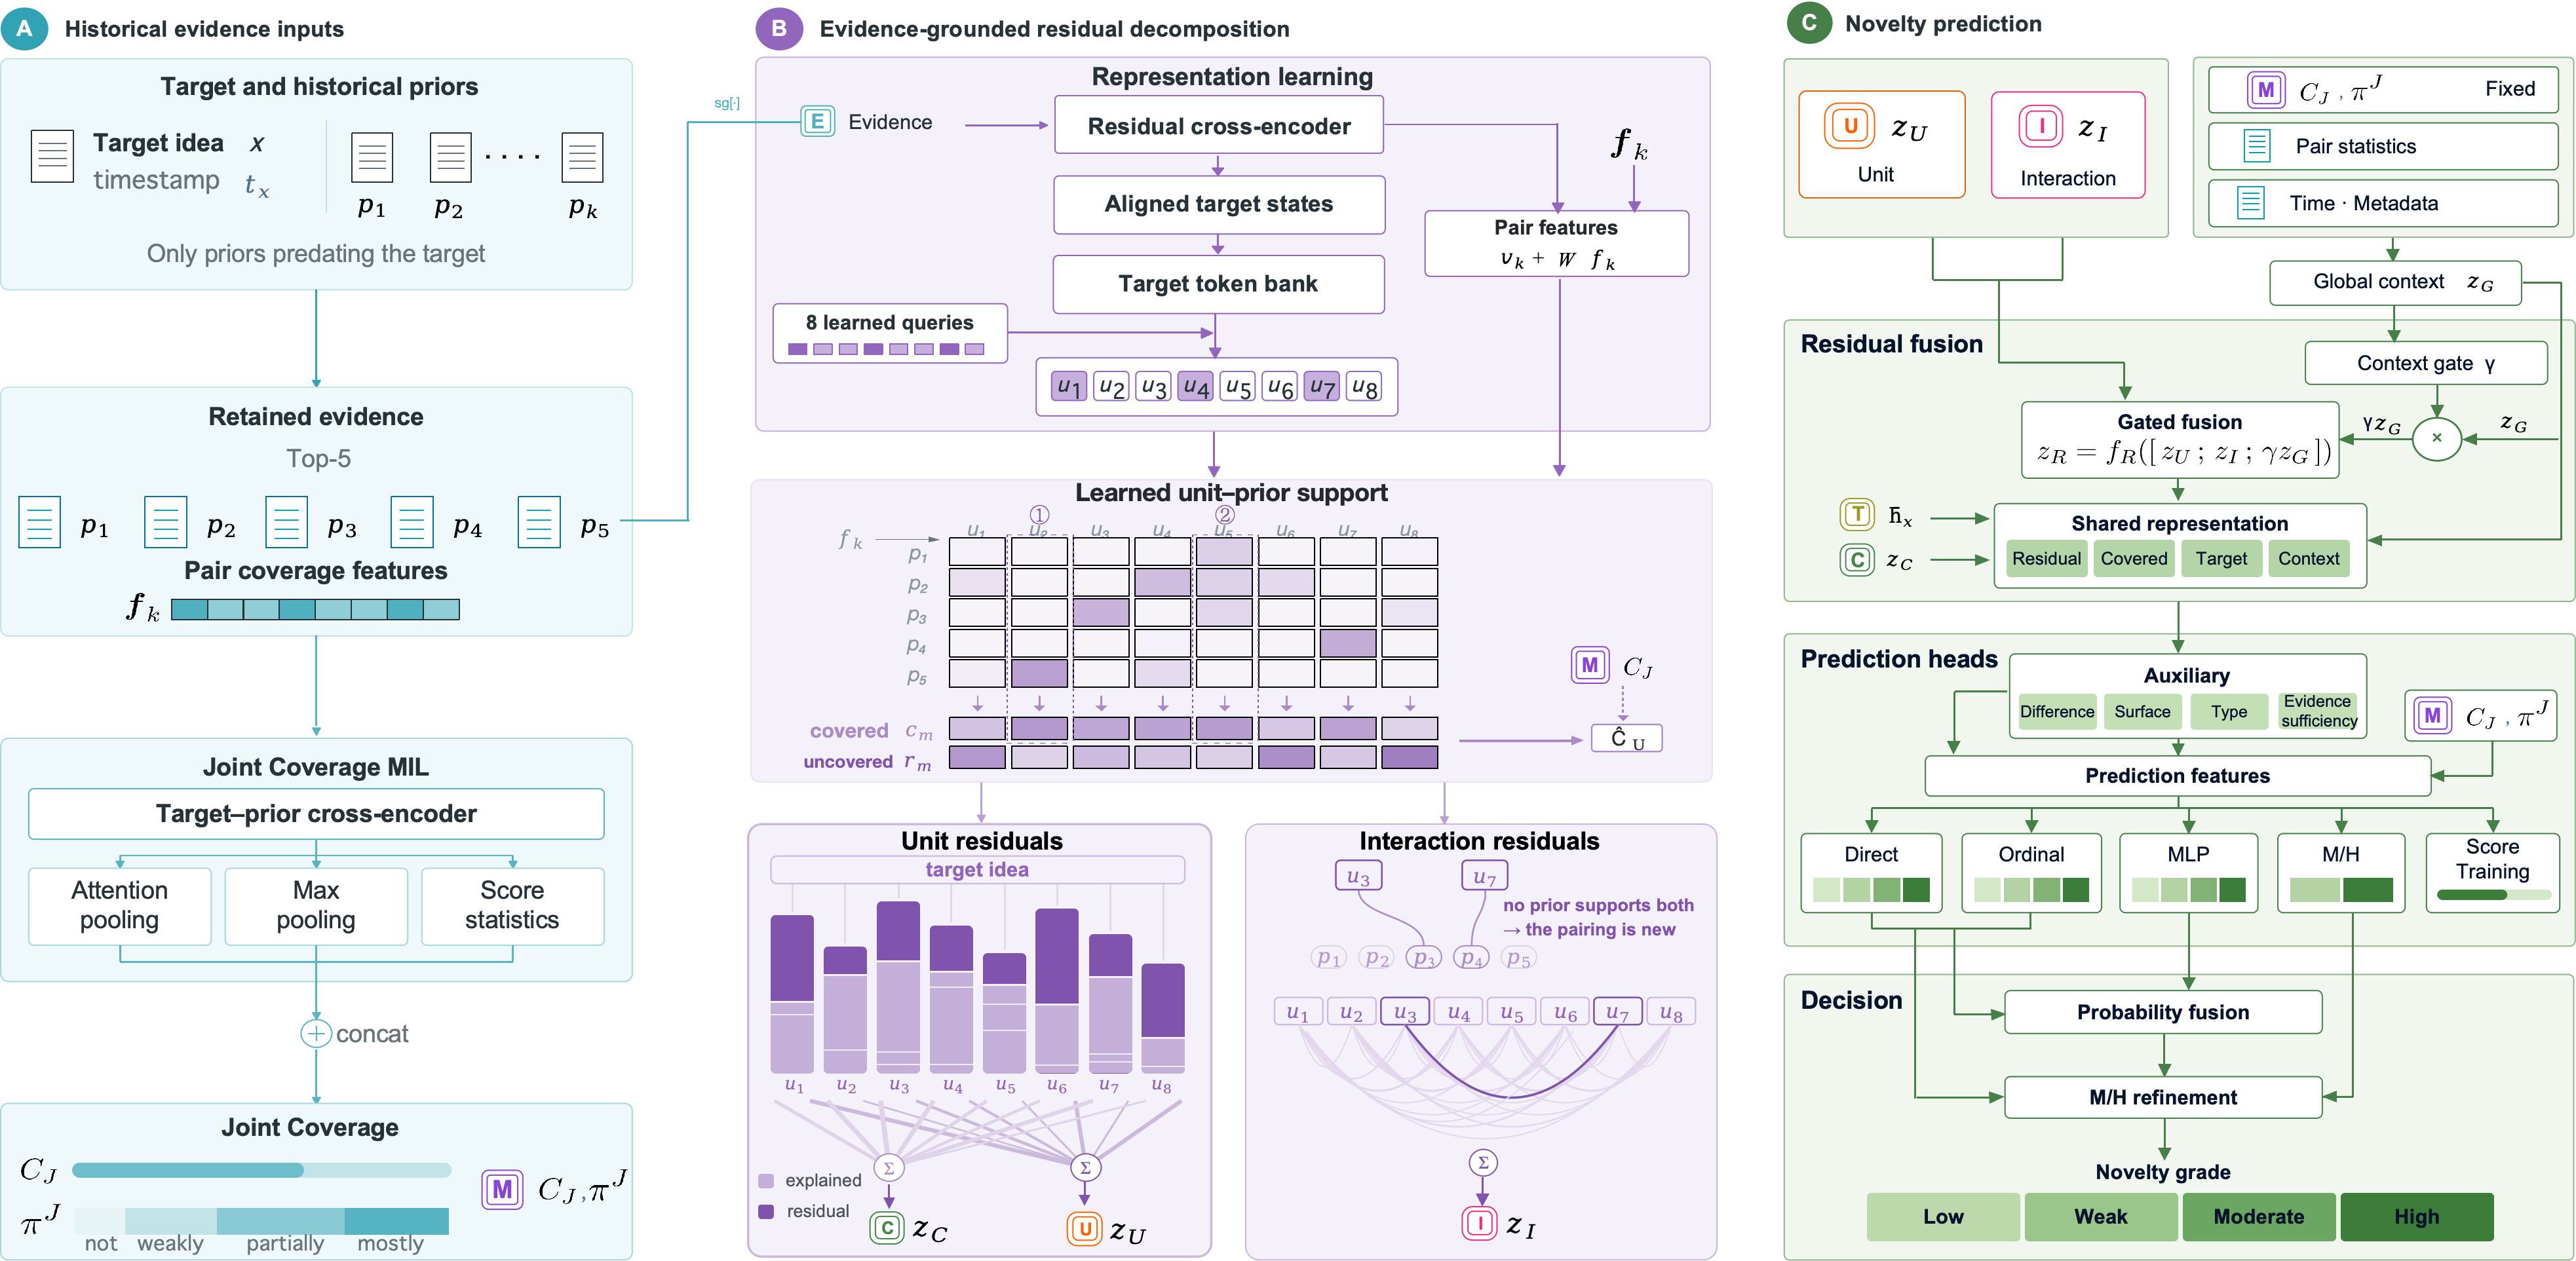
\includegraphics[width=\textwidth]{pic/framework.png}
\caption{Overview of EGRD. \textbf{(A)} Only priors predating the target are
admissible; the retained top-$K$ evidence carries pair coverage features
$\boldsymbol{f}_k$, and a multiple-instance model over target--prior pairs
predicts joint coverage $C_J$ and its four-class distribution
$\boldsymbol{\pi}^{J}$. These outputs enter the later stages as fixed inputs,
marked $\mathrm{sg}[\cdot]$. \textbf{(B)} A
residual cross-encoder builds a target token bank, which $M$ learned queries
partition into semantic units $\boldsymbol{u}_m$. A learned support matrix
$A_{km}$ aligns each unit with each prior; noisy-OR over priors gives unit
coverage $c_m$, and the complementary residual $r_m$ weights the units into
$\boldsymbol{z}_U$, with the covered part pooled into $\boldsymbol{z}_C$. The
support matrix also yields co-support $b_{ij}$, so a unit pair that no single
prior supports jointly contributes to the interaction residual
$\boldsymbol{z}_I$. \textbf{(C)} A gate modulates global context within
residual fusion; the fused representation, the covered and target
representations, and global context form a shared representation.
Auxiliary predictions and joint coverage further inform the novelty branches. Direct and ordinal probabilities enter both the fused distribution
and the moderate-to-high refinement, while the continuous score head supplies
auxiliary training supervision and is excluded from the inference-time
grading rule.}
\label{fig:framework}
\end{figure}

\subsection{Stage A: Historical Evidence Inputs}
\label{sec:method-evidence}

Stage~A assembles historical evidence and estimates how much of the target
idea that evidence collectively covers. Given a target idea $x$ with timestamp
$t_x$, we restrict candidate priors to
$\mathcal{P}_x=\{p_k\mid t_{p_k}<t_x\}$, where $t_{p_k}$ denotes the timestamp
of prior idea $p_k$. We retain the top-$K$ ranked priors, or all candidates if
fewer are available, to form the evidence set
$\mathcal{E}_x\subseteq\mathcal{P}_x$ ($K=5$ in our experiments). Each retained
prior $p_k$ is associated with coverage features $\boldsymbol{f}_k$ for the
target--prior pair.

To estimate coverage across the evidence set, we use a multiple-instance
model \citep{ilse2018attentionmil}. A cross-encoder encodes each target--prior
pair, and the model aggregates the pair representations through attention
pooling and maximum pooling. The pooled representations are concatenated
with evidence-score statistics to predict joint coverage $C_J$ and a
four-class coverage distribution $\boldsymbol{\pi}^{J}$.
Appendix~\ref{app:method-evidence} specifies the pair-scoring rule and the joint
model. The retained evidence, pair features, and coverage predictions serve
as fixed inputs to Stages~B and~C, grounding the residual decomposition and
providing coverage information for novelty prediction.

We summarize the evidence set in a global context vector $\boldsymbol{z}_G$,
a learned projection of twenty-one scalars---the scaled target timestamp,
pair-score statistics over $\mathcal{E}_x$, and the joint coverage score,
entropy, and distribution $\boldsymbol{\pi}^{J}$---concatenated with
embeddings of two target facets (aspect and contribution type).
Apart from the timestamp and the facets, $\boldsymbol{z}_G$ is a
re-encoding of the Stage~A outputs, and Stage~C consumes it as a summary of
what the evidence collectively establishes.

\subsection{Stage B: Evidence-Grounded Residual Decomposition}
\label{sec:method-decomposition}

Stage~B decomposes the target into semantic units and estimates their support
from the retained evidence. It represents the unexplained contribution through
two complementary components: unit residuals for content with limited
historical support, and interaction residuals for combinations with limited
joint support from any single prior.

\paragraph{Semantic decomposition.}
We use a residual cross-encoder initialized from the Stage~A model and trained
separately from it. For each target--prior pair, the encoder produces a pooled
representation $\boldsymbol{v}_k$, which we augment with projected pair
coverage features:
$\widetilde{\boldsymbol{v}}_k=\boldsymbol{v}_k+f_P(\boldsymbol{f}_k)$.
To obtain a shared representation of the target, we average its contextual
token states at matching positions across valid pairs, forming a token bank
$\{\boldsymbol{h}_j\}_{j=1}^{N}$, where $N$ is the number of target tokens.
We then use $M$ learned queries $\boldsymbol{q}_m$ to softly assign these tokens
to semantic units \citep{locatello2020slot} ($M=8$ in our experiments).
Queries compete for each token through a softmax over units; the resulting
assignments are then normalized over tokens within each unit:
\begin{equation}
 B_{mj}=\operatorname{softmax}_{m}
 \left(\frac{\boldsymbol{q}_m^\top\boldsymbol{h}_j}{\sqrt d}\right),
 \quad
 \alpha_{mj}=\frac{B_{mj}}{\sum_{j'\in\mathcal{V}}B_{mj'}+\varepsilon},
 \quad
 \boldsymbol{u}_m=\sum_{j\in\mathcal{V}}\alpha_{mj}\boldsymbol{h}_j.
 \label{eq:semantic-units}
\end{equation}
The units have no predefined semantic roles. A learned activity score
$v_m=\sigma(\boldsymbol{w}_v^\top\boldsymbol{u}_m+b_v)$ controls each unit's
contribution, while regularization discourages redundant token assignments.

\paragraph{Evidence-aligned unit residuals.}
\label{sec:method-unit-residual}
We estimate how strongly each prior $p_k$ supports each unit $\boldsymbol{u}_m$
through a learned support matrix:
\begin{equation}
 A_{km}=\sigma\left(f_A([
 \boldsymbol{u}_m;\widetilde{\boldsymbol{v}}_k;
 \boldsymbol{u}_m\odot\widetilde{\boldsymbol{v}}_k;
 |\boldsymbol{u}_m-\widetilde{\boldsymbol{v}}_k|;\boldsymbol{f}_k])\right),
 \label{eq:unit-support}
\end{equation}
where $f_A$ is an MLP. Support is estimated separately for every target--prior
pair, so different priors can account for different units. For
$n=|\mathcal{E}_x|$ retained priors, noisy-OR aggregates support across priors
into unit coverage $c_m$. Its complement, weighted by unit activity, defines
the residual weight $r_m$:
\begin{equation}
 c_m=1-\prod_{k=1}^{n}(1-A_{km}),\qquad
 r_m=v_m(1-c_m),\qquad
 \boldsymbol{z}_U=\frac{1}{M}\sum_m r_m\boldsymbol{u}_m.
 \label{eq:unit-residual}
\end{equation}
Noisy-OR lets several partially relevant priors jointly cover a unit that none
of them covers alone. We use it as a differentiable aggregation rule, not as a
claim that the priors are independent sources of support
(Appendix~\ref{app:method-representations}).
An active unit with little historical support receives a large residual
weight in $\boldsymbol{z}_U$. We normalize by the fixed number of units $M$
rather than by $\sum_mr_m$, so that the pooled representation retains the total
residual mass instead of dividing it away. We also pool
the supported content as
$\boldsymbol{z}_C=M^{-1}\sum_m v_mc_m\boldsymbol{u}_m$.
To connect unit coverage to supervision, a learned, activity-weighted pooling
of $c_m$ reconstructs joint coverage $\widehat C_U$, supervised by annotated
coverage and the fixed Stage~A prediction. The entries of the support matrix
are latent strengths learned without unit-level alignment labels.

\paragraph{Interaction residuals.}
\label{sec:method-interaction}
Units that are individually covered may still form a new combination. For
each unit pair $i<j$, an MLP maps their concatenation, elementwise product,
and absolute difference to an interaction representation
$\boldsymbol{t}_{ij}$, and a sigmoid head predicts its strength $g_{ij}$.
We measure historical co-support by the largest product of the two units'
support strengths within a single prior. The co-support score $b_{ij}$,
interaction residual weight $r_{ij}$, and pooled representation are
\begin{equation}
 b_{ij}=\max_k A_{ki}A_{kj},\qquad
 r_{ij}=g_{ij}(1-b_{ij}),\qquad
 \boldsymbol{z}_I=\sum_{i<j}\eta_{ij}r_{ij}\boldsymbol{t}_{ij},
 \label{eq:interaction-residual}
\end{equation}
where the learned attention $\eta_{ij}$ includes a
$\log(r_{ij}+\varepsilon)$ bias that favors pairs with larger residual
weights. When different priors support the two units but no single prior
strongly supports both, their unit residuals can be small while their
interaction residual remains large, provided that $g_{ij}$ is high.
An auxiliary classifier on $\boldsymbol{z}_I$ is trained with idea-level
labels for nontrivial combinations. Co-support serves as a proxy for an
existing combination: a prior that supports both units need not cover the
specific way they are combined in the target.
Appendix~\ref{app:method-representations} provides the detailed pooling
equations.

\subsection{Stage C: Novelty Prediction}
\label{sec:method-prediction}

Stage~C predicts an ordered novelty grade from the residual representations
and the evidence context. To account for evidence availability and uncertainty,
we condition residual fusion on the global context $\boldsymbol{z}_G$ defined
in Section~\ref{sec:method-evidence}. A learned gate $\gamma$ takes
$\boldsymbol{z}_U$, $\boldsymbol{z}_I$, $\boldsymbol{z}_G$, and the entropy of
the Stage~A coverage prediction as inputs and scales the context within the
residual branch:
\begin{equation}
 \boldsymbol{z}_R=f_R([\boldsymbol{z}_U;\boldsymbol{z}_I;
                       \gamma\boldsymbol{z}_G]),\qquad
 \boldsymbol{h}=\operatorname{LayerNorm}([
 \boldsymbol{z}_R;\boldsymbol{z}_C;\bar{\boldsymbol{h}}_x;\boldsymbol{z}_G]),
 \label{eq:residual-fusion}
\end{equation}
where $\bar{\boldsymbol{h}}_x$ is obtained by masked mean pooling over the target token bank.
The shared representation $\boldsymbol{h}$ retains the covered content,
the target representation, and a direct path for global context. The gate
therefore controls context only within residual fusion.

Auxiliary heads predict substantive difference, surface change, evidence
sufficiency, and residual type. These predictions, together with
$\boldsymbol{h}$ and joint coverage, form the inputs to three novelty
branches: a direct linear classifier, a cumulative ordinal head that models
grade order, and a two-layer MLP classifier. Each branch produces a
four-class distribution, and their convex mixture determines an initial
grade. A moderate-to-high refinement upgrades an initial \textsc{moderate}
prediction when a weighted combination of the direct and ordinal
\textsc{high}-class probabilities and a separate binary-head score exceeds
a threshold. The mixture weights and refinement threshold are selected on
development data and fixed for testing
(Appendix~\ref{app:method-heads}). A separate continuous novelty head provides
auxiliary supervision during training; its output is not used in the
inference-time grading rule.

\subsection{Training Objective}
\label{sec:method-learning}

We initialize the residual encoder from the Stage~A joint-coverage checkpoint
and jointly optimize it with the decomposition and prediction modules in
Stages~B and~C, while keeping the Stage~A models fixed. The objective combines
classification of the novelty grade and the residual type, supervision of a
family of annotated scalar quantities, and regularization of the
decomposition.

Let $\mathcal{A}=\{\Delta,S,E,C,\nu\}$ index the annotated scalars---the
substantive difference, surface change, and evidence sufficiency read off the
auxiliary heads, the reconstructed coverage $\widehat C_U$, and the continuous
novelty score. Each contributes a smooth-$L_1$ level loss $\mathcal{L}_a$
against its annotation. Level losses alone leave these heads free to settle on
the median of their target, so we also supervise their order: the ranking terms
of $\Delta$, $S$, $E$, and $C$ are collected into a single
$\mathcal{L}_{\mathrm{rank}}$, while the novelty score carries its own ranking
term inside $\mathcal{L}_{\nu}$. The objective is
\begin{equation}
 \mathcal{L}=\sum_{a\in\mathcal{A}}\lambda_{a}\mathcal{L}_{a}
 +\lambda_{\mathrm{rank}}\mathcal{L}_{\mathrm{rank}}
 +\lambda_{\mathrm{nov}}\mathcal{L}_{\mathrm{nov}}
 +\lambda_{\mathrm{type}}\mathcal{L}_{\mathrm{type}}
 +\lambda_{\mathrm{dec}}\mathcal{L}_{\mathrm{dec}}
 +\lambda_{\mathrm{var}}\mathcal{L}_{\mathrm{var}}.
 \label{eq:training-objective}
\end{equation}
Here $\mathcal{L}_{\mathrm{nov}}$ supervises the three novelty branches, their
fused distribution, and the moderate-to-high head, and
$\mathcal{L}_{\mathrm{type}}$ supervises residual categories and nontrivial
combinations. Beyond its level loss, the coverage term $\mathcal{L}_{C}$ adds a
consistency loss against the fixed Stage~A prediction, assigning less
consistency weight to predictions with higher entropy.
$\mathcal{L}_{\mathrm{dec}}$ regularizes the decomposition against redundant
token assignments and unused units, and $\mathcal{L}_{\mathrm{var}}$ is a
variance floor that keeps the unit coverages from coinciding.
Appendix~\ref{app:method-training} defines each term and reports the
coefficients $\lambda$.

% Experiments. Main results on IdeaDelta, then the RINoBench transfer as a
% separate subsection (frozen checkpoint, expert labels, different evidence
% budget --- not part of the main comparison), then ablation and case study.
% Every number is copied unchanged from the recorded artifacts; provenance
% comments live beside the table that carries them. Setup, the transfer
% protocol, seed variability and the sweep protocol notes are in the appendix.

\section{Experiments}
\label{sec:experiments}

The evaluation asks three things: whether the decomposition beats prompting a
language model on the same evidence (\S\ref{sec:exp-main}), whether what it
learns survives labels it was not trained on (\S\ref{sec:exp-transfer}), and
what its predictions depend on (\S\ref{sec:exp-ablation},
\S\ref{sec:exp-case}). The last is answerable only because the evidence is
supplied rather than retrieved: on the \textsc{IdeaDelta} test split every
system but one reads the same five admissible priors per target. All rows report
Accuracy, Macro-F1, QWK and MAE; Appendix~\ref{app:setup} gives the splits,
hyperparameters and scoring code.

\subsection{Main results}
\label{sec:exp-main}

\begin{table}[t]
\centering
\scriptsize
\setlength{\tabcolsep}{2.6pt}
\renewcommand{\arraystretch}{1.0}
\caption{Baselines and our model on the IdeaDelta evaluation set, 3{,}352 ideas,
split by domain. A majority-class predictor scores $0.312$ Accuracy on Graph ML,
$0.356$ on computer vision and $0.328$ on time series, with QWK $0$ by
construction.}
\label{tab:main}
\resizebox{\textwidth}{!}{%
\begin{tabular}{@{}ll rrrr rrrr rrrr@{}}
\toprule
& & \multicolumn{4}{c}{Graph ML} & \multicolumn{4}{c}{Computer vision} & \multicolumn{4}{c}{Time series} \\
\cmidrule(lr){3-6}\cmidrule(lr){7-10}\cmidrule(lr){11-14}
System & Backbone
& Accuracy & Macro-F1 & QWK & MAE $\downarrow$
& Accuracy & Macro-F1 & QWK & MAE $\downarrow$
& Accuracy & Macro-F1 & QWK & MAE $\downarrow$ \\
\midrule
% Dense RAG rows: results/llm_eval/rag_ab/, the {,cv_,time_series_} runs for
% Qwen3.5 and the {luna,flash}_<domain>_ runs for the other two backbones.
% Priors come from query-time dense retrieval (bge-large-en-v1.5 over every
% canonical idea with an earlier date) instead of the stored candidate lists,
% which are ordered by the gold coverage label. Built by
% baseline/dense_rag/build_dense_retrieval.py.
Dense RAG, 5 priors & Qwen3.5
& 0.360 & 0.217 & 0.129 & 0.867
& 0.367 & 0.248 & 0.191 & 0.801
& 0.318 & 0.248 & 0.190 & 0.954 \\
& deepseek-flash
& 0.371 & 0.236 & 0.152 & 0.842
& 0.369 & 0.232 & 0.154 & 0.801
& 0.326 & 0.224 & 0.205 & 0.919 \\
& gpt-5.6-luna
& 0.362 & 0.262 & 0.253 & 0.810
& 0.372 & 0.289 & 0.267 & 0.787
& 0.346 & 0.295 & 0.292 & 0.883 \\
\addlinespace
Direct, 5 priors & Qwen3.5
& 0.300 & 0.266 & 0.319 & 0.925
& 0.308 & 0.264 & 0.300 & 0.876
& 0.291 & 0.283 & 0.327 & 0.956 \\
& deepseek-flash
& 0.438 & 0.444 & 0.558 & 0.706
& 0.409 & 0.418 & 0.521 & 0.728
& 0.416 & 0.415 & 0.560 & 0.716 \\
& gpt-5.6-luna
& 0.432 & 0.439 & 0.579 & 0.657
& 0.420 & 0.430 & 0.561 & 0.661
& 0.445 & 0.436 & 0.576 & 0.653 \\
\addlinespace
Schopf 2-stage & Qwen3.5
& 0.324 & 0.286 & 0.335 & 0.831
& 0.346 & 0.293 & 0.338 & 0.777
& 0.344 & 0.333 & 0.413 & 0.793 \\
& deepseek-flash
& 0.443 & 0.458 & 0.560 & 0.639
& 0.416 & 0.411 & 0.501 & 0.676
& 0.442 & 0.447 & 0.553 & 0.654 \\
& gpt-5.6-luna
& 0.391 & 0.377 & 0.487 & 0.698
& 0.393 & 0.364 & 0.458 & 0.683
& 0.392 & 0.379 & 0.512 & 0.688 \\
\addlinespace
UKPLab 3-stage & Qwen3.5
& 0.280 & 0.161 & 0.125 & 0.928
& 0.289 & 0.150 & 0.106 & 0.873
& 0.274 & 0.180 & 0.132 & 0.973 \\
& deepseek-flash
& 0.351 & 0.267 & 0.301 & 0.761
& 0.376 & 0.272 & 0.259 & 0.741
& 0.386 & 0.289 & 0.290 & 0.727 \\
& gpt-5.6-luna
& 0.318 & 0.226 & 0.266 & 0.800
& 0.367 & 0.248 & 0.304 & 0.721
& 0.365 & 0.267 & 0.296 & 0.743 \\
\addlinespace
% GraphMind rows: results/llm_eval/baseline/{qwen35,deepseek_flash,gpt5.6_luna}.
% The Qwen run covers the evaluation set directly; the deepseek and gpt runs
% carry their own idea ids and their own gold labels, so their targets are
% matched to the evaluation set by target text and rescored against its labels,
% the ones every other row uses. Coverage: Graph ML 771/850 and 783/850,
% computer vision 1137/1137, time series 1120/1190.
GraphMind & Qwen3.5
& 0.264 & 0.205 & 0.154 & 1.027
& 0.264 & 0.182 & 0.108 & 0.959
& 0.244 & 0.204 & 0.155 & 1.051 \\
& deepseek-flash
& 0.291 & 0.227 & $-$0.007 & 1.095
& 0.342 & 0.266 & 0.154 & 0.971
& 0.365 & 0.249 & 0.159 & 0.916 \\
& gpt-5.6-luna
& 0.289 & 0.255 & 0.046 & 1.003
& 0.381 & 0.328 & 0.304 & 0.755
& 0.380 & 0.327 & 0.305 & 0.750 \\
\addlinespace
DeepReviewer & DeepReviewer-7B
& 0.294 & 0.237 & 0.034 & 0.965
& 0.325 & 0.235 & $-$0.043 & 0.972
& 0.296 & 0.222 & $-$0.017 & 0.964 \\
\addlinespace
\textbf{EGRD (ours)} & ---
& \textbf{0.799} & \textbf{0.801} & \textbf{0.909} & \textbf{0.201}
& \textbf{0.761} & \textbf{0.767} & \textbf{0.882} & \textbf{0.242}
& \textbf{0.789} & \textbf{0.776} & \textbf{0.898} & \textbf{0.215} \\
\bottomrule
\end{tabular}}
\end{table}

We compare against a \emph{direct} single call; two multi-stage prompt chains,
\emph{Schopf 2-stage}, the evaluation prompt accompanying RINoBench
\citep{schopf2026rinobench}, and \emph{UKPLab 3-stage}
\citep{afzal2026beyond}; \emph{GraphMind} \citep{dasilva2025graphmind}, which
labels each prior as supporting or contrasting before rating;
\emph{DeepReviewer-7B} \citep{zhu2025deepreview}, a reviewer model fine-tuned on
paper review; and a \emph{dense RAG} group running the \emph{direct} call on
five priors it retrieves itself by dense similarity to the target. All but
DeepReviewer-7B appear once per backbone. Table~\ref{tab:main} reports every
system on the \textsc{IdeaDelta} evaluation set.

Prompt chaining has backbone-dependent effects. Relative to the direct call,
Schopf 2-stage improves Accuracy and QWK in all three domains on Qwen3.5,
but provides no QWK gain on deepseek-flash and reduces both metrics on
gpt-5.6-luna. UKPLab 3-stage and GraphMind fall below the direct call on
both metrics across all nine backbone--domain combinations. These results
show that adding intermediate judgments does not consistently improve novelty
assessment.

Replacing supplied priors with dense retrieval reduces Macro-F1 and QWK
across all nine backbone--domain combinations. Accuracy remains between
$0.318$ and $0.372$, near the majority-class baselines, even though it increases
on Qwen3.5. Thus, relevant evidence retrieved by generic similarity does not
recover the benefit of the supplied target--prior relationships. This
complements the random-prior intervention in
Appendix~\ref{app:dataset-validity}, which tests whether evidence is on topic:
the dense-retrieval comparison additionally tests whether topical relevance
alone suffices.

EGRD leads every baseline in every domain by $0.34$ Accuracy or more over the
best baseline of that domain, a margin that barely varies across the three,
unlike the baselines' ranking among each other. DeepReviewer-7B transfers least:
its ordinal agreement is near zero in all three domains and negative in two, so
fine-tuning on paper review does not recover the grade ordering here.

\subsection{Transfer Evaluation}
\label{sec:exp-transfer}

To evaluate transfer beyond \textsc{IdeaDelta}'s model-generated labels, we
test the frozen checkpoint from Table~\ref{tab:main} on RINoBench
\citep{schopf2026rinobench}, which contains 277 expert-rated ideas spanning
machine learning. Table~\ref{tab:transfer} reports agreement with expert ratings
mapped to four ordinal grades. Appendix~\ref{app:transfer} details the data,
label mapping, inference procedure, and baseline evaluation.

\begin{table}[t]
\centering
\footnotesize
\setlength{\tabcolsep}{5pt}
\renewcommand{\arraystretch}{1.0}
\caption{Results on RINoBench with expert ratings mapped to four ordinal grades.}
\label{tab:transfer}
\begin{tabular}{@{}p{5.1cm}rrrr@{}}
\toprule
System & Accuracy & Macro-F1 & QWK & MAE $\downarrow$ \\
\midrule
\multicolumn{5}{@{}l}{\emph{Same Qwen3.5 backbone, zero-shot}} \\
Qwen3.5 & 0.3574 & 0.2244 & 0.1451 & 0.7726 \\
GraphMind & 0.3357 & 0.2281 & 0.1469 & 0.7653 \\
UKPLab 3-stage & 0.3466 & 0.1892 & 0.0808 & \textbf{0.7220} \\
\addlinespace
\multicolumn{5}{@{}l}{\emph{Released predictions of the benchmark authors, folded to four levels}} \\
GPT-5 & 0.3646 & 0.2457 & 0.0955 & 0.8051 \\
o3 & 0.3971 & 0.2370 & 0.0606 & 0.8087 \\
gpt-oss-120b & 0.4152 & 0.2249 & 0.0392 & 0.8375 \\
Llama-3.1-8B-Instruct & 0.3755 & 0.1961 & $-$0.0011 & 0.8773 \\
DeepSeek-R1 & \textbf{0.4224} & 0.1873 & 0.0283 & 0.8700 \\
Llama-4-Scout-17B-16E & 0.4116 & 0.1864 & 0.0215 & 0.8809 \\
Llama-3.3-70B-Instruct & 0.4188 & 0.1531 & 0.0051 & 0.9025 \\
\addlinespace
\multicolumn{5}{@{}l}{\emph{Reviewer model fine-tuned on paper review, local weights}} \\
DeepReviewer-7B & 0.1913 & 0.1425 & 0.0145 & 1.3610 \\
\addlinespace
\textbf{EGRD (ours)} & 0.4152 & \textbf{0.3407} & \textbf{0.2245} & 0.8087 \\
\bottomrule
\end{tabular}
\end{table}

EGRD achieves the highest Macro-F1 ($0.3407$) and QWK ($0.2245$),
although other systems lead on Accuracy and MAE. The folded label distribution
places $41.5\%$ of ideas in one class, so a constant prediction already attains
$0.4152$ Accuracy while yielding zero QWK. EGRD reaches the same Accuracy
with predictions distributed across all four grades: $16/36/76/149$, against
gold counts of $15/60/87/115$. Its higher Macro-F1 and QWK therefore provide
complementary evidence of agreement with expert judgments.

Transfer remains limited by domain and label differences. Only 30 of the 277
RINoBench ideas fall within \textsc{IdeaDelta}'s three fields; the remaining
247 test generalization beyond the task-specific training domains. Moreover,
mapping five expert levels to four grades merges the top two levels and
prevents evaluation of distinctions within that merged class. We interpret
these results as partial transfer from model-generated supervision to expert
judgments.

\subsection{Ablation}
\label{sec:exp-ablation}

% Source values and plotting code: scripts/plot_ablation.py.
\begin{figure}[t]
\centering
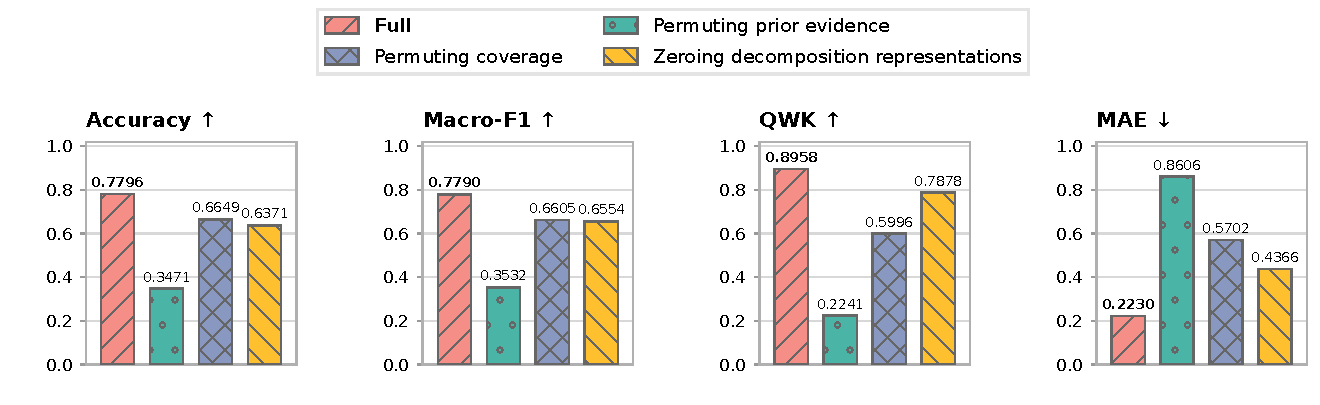
\includegraphics[width=\textwidth]{pic/ablation/pipeline_stages.pdf}
\caption{Pipeline-stage ablations on IdeaDelta. Full is the unablated checkpoint
of Table~\ref{tab:main}; each intervention is applied at inference without
retraining. Arrows indicate the preferred direction for each metric.}
\label{fig:ablation-pipeline}
\end{figure}

\begin{figure}[t]
\centering
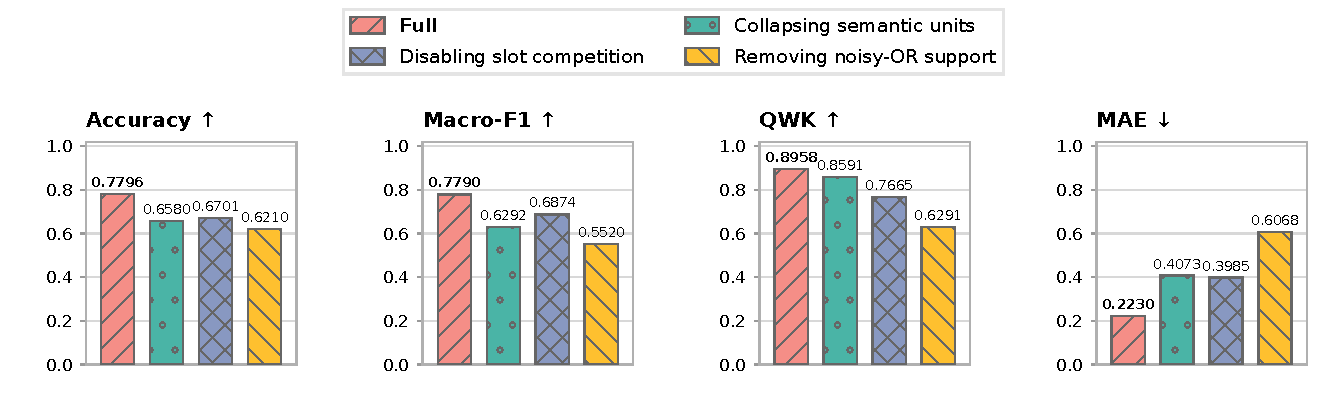
\includegraphics[width=\textwidth]{pic/ablation/decomposition_design.pdf}
\caption{Decomposition-design ablations on IdeaDelta. Each variant is retrained
without the corresponding component and compared with the same Full model.
Arrows indicate the preferred direction for each metric.}
\label{fig:ablation-decomposition}
\end{figure}

Because the supplied evidence can be intervened on with the target held fixed,
we can test what the trained model's predictions actually depend on. The three
pipeline interventions in Figure~\ref{fig:ablation-pipeline} cut the chain at
successive points.
\textbf{Permuting prior evidence} shuffles the retrieved prior texts across
targets, breaking the correspondence between each target and its evidence in
Stage~A. \textbf{Permuting coverage} shuffles only the joint coverage score
produced by Stage~A while leaving every prior text in place.
\textbf{Zeroing decomposition representations} sets the unit residual $\boldsymbol{z}_U$,
interaction residual $\boldsymbol{z}_I$ and covered-content representation
$\boldsymbol{z}_C$ to zero, removing these three outputs of Stage~B
together. All three reduce performance on
every metric.

Permuting prior evidence causes the largest loss across all four metrics,
establishing target--prior correspondence as a critical basis for the model's
predictions. Permuting coverage preserves the prior texts but sharply reduces
ordinal agreement and increases grade errors, showing that the remaining inputs
cannot compensate for a corrupted coverage signal. Zeroing decomposition
representations produces more incorrect predictions than permuting coverage,
but smaller grade errors on average. Together, these
results suggest complementary roles for coverage in maintaining ordinal
agreement and decomposition representations in assigning the exact grade.

Figure~\ref{fig:ablation-decomposition} shows that the three mechanisms inside
the decomposition are not interchangeable; each removal degrades a different
part of the prediction.
\textbf{Collapsing semantic units} from eight to one costs on Accuracy, Macro-F1
and MAE while QWK barely moves.
\textbf{Disabling slot competition}, which removes the softmax through which the
units compete for each token, reverses that pattern: QWK falls while MAE stays
where collapsing the units left it.
\textbf{Removing noisy-OR support} costs the most of the three on all four
metrics and most of all on the rank-sensitive ones.

We also conduct parameter sensitivity experiments using the default configuration,
with detailed results reported in
Appendix~\ref{app:sensitivity}.

\subsection{Case study}
\label{sec:exp-case}

% Figure: figures/case_study/make_figure.py, from figures/case_study/pull_full.npz
% and figures/case_study/cases.json. Cases CI_26954 (low), CI_18669 (moderate),
% CI_18985 (high); every number below is read off those two artifacts.
\begin{figure}[t]
\centering
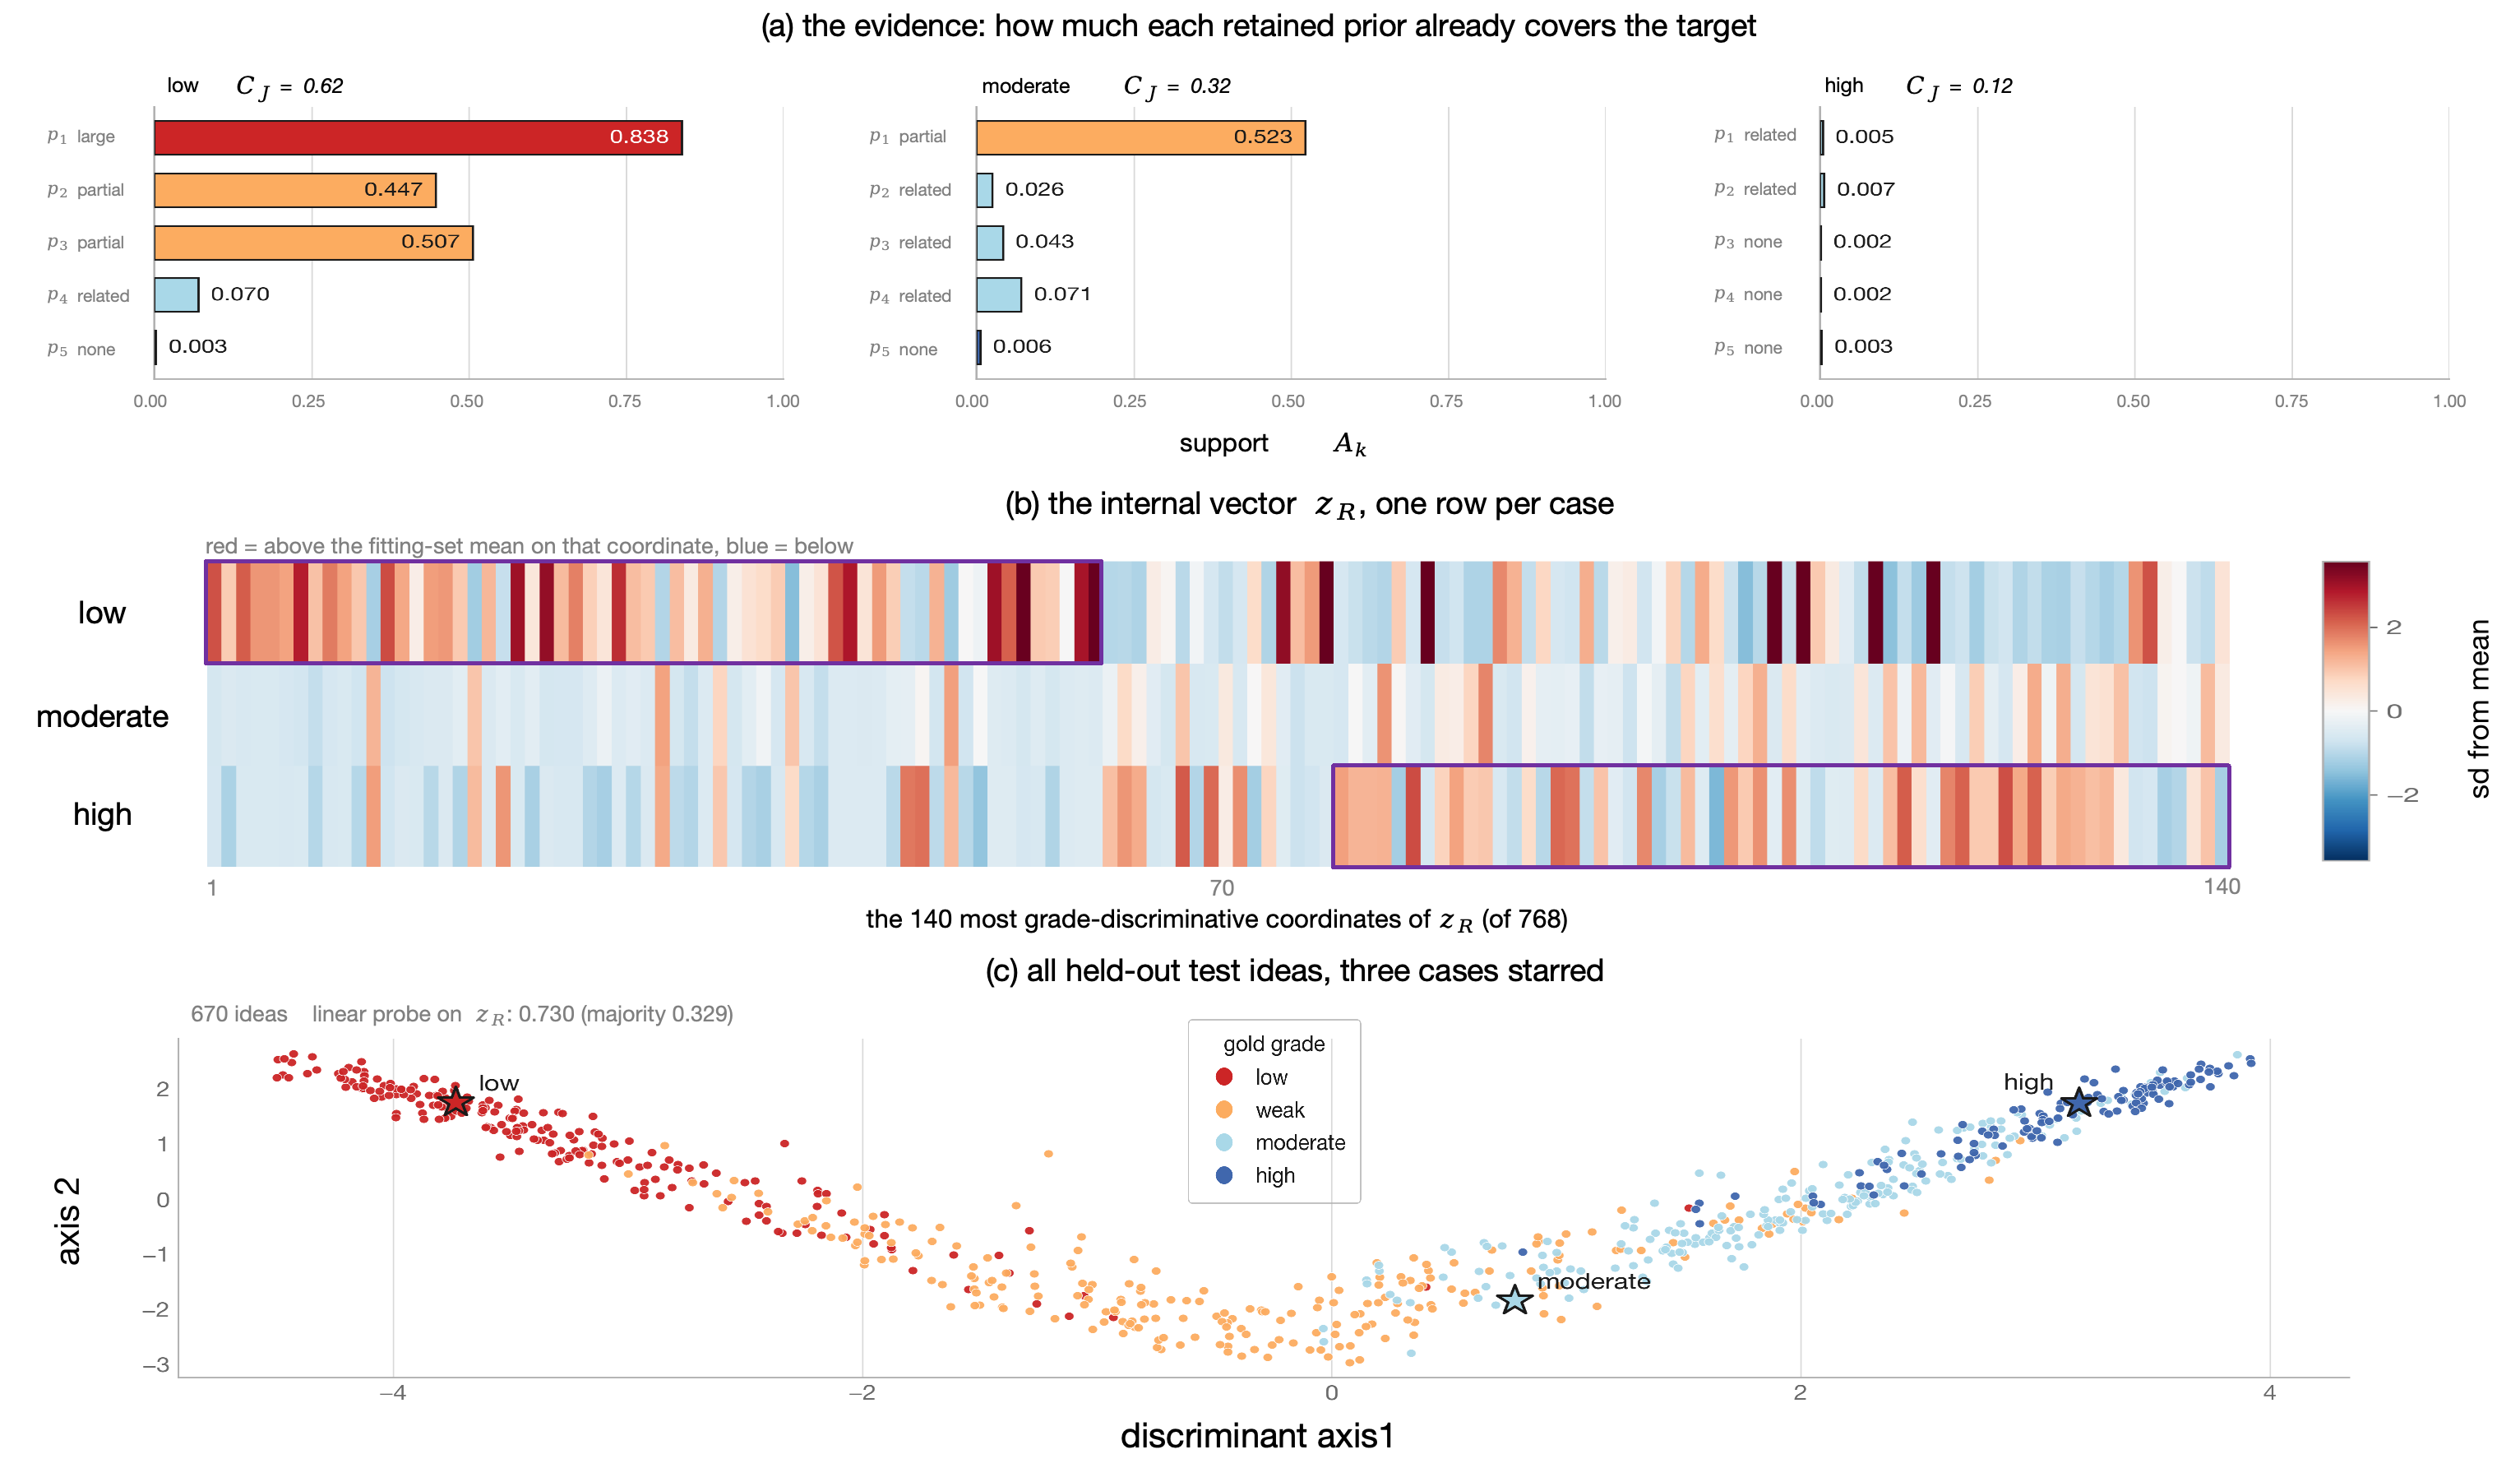
\includegraphics[width=\textwidth]{pic/case_study.png}
\caption{Three test targets, graded low, moderate and high, traced through the
model. \textbf{(a)} The support $A_k$ assigned to each retained prior, against
the coverage label the annotation carries; $C_J$ is the predicted joint
coverage. \textbf{(b)} The residual representation $\boldsymbol{z}_R$ of each
case, as deviations from the fitting-set mean. \textbf{(c)} $\boldsymbol{z}_R$ for
every held-out test idea, coloured by gold grade, the three cases starred.}
\label{fig:case-study}
\end{figure}

Figure~\ref{fig:case-study} traces three correctly predicted cases from
evidence coverage to residual representations. Joint coverage decreases from
the low- to the high-novelty case, while their residual embeddings show
distinct patterns. In the supervised discriminant projection, held-out ideas
are broadly ordered by novelty along the first axis, with overlap between
adjacent grades; the three cases occupy regions consistent with their labels.
These examples illustrate the association between evidence coverage and
novelty-sensitive representations. Appendix~\ref{app:case-study} provides
visualization details.

\section{Conclusion}
\label{sec:conclusion}

EGRD grades an idea by what an explicit set of admissible priors leaves over,
estimating coverage at the level of semantic units and predicting the grade from
the residuals that survive alignment with the evidence. Supplying that evidence
rather than retrieving it is what lets the design be checked: permuting the
priors lowers Accuracy to the majority-class band, removing noisy-OR
aggregation costs more on every metric than any other change to the
decomposition, and a cross-validated probe finds grade information linearly
accessible in the residual representation. EGRD outperforms every
prompted baseline we evaluate, whether it reads the supplied priors or selects
its own. On expert labels, the ordering transfers while the level does not
(App.~\ref{app:limitations}).


\bibliography{iclr2027_conference}
\bibliographystyle{iclr2027_conference}

\appendix

\section{Related Work}
\label{app:related}

\paragraph{Automated research and idea generation.} Language models are
increasingly used to carry out parts of the research process itself.
\citet{wang2024scimon} retrieve inspirations from past literature and optimise
explicitly for novelty by comparing a candidate against prior papers;
\citet{baek2025researchagent} refine proposals against a set of LLM reviewing
agents that give structured feedback along several dimensions; and
\citet{lu2024aiscientist} and \citet{schmidgall2025agentlab} close the loop
from ideation through experiments to a
written paper and a simulated review. \citet{si2025llmideas} evaluate what such
pipelines produce, finding the generated ideas rated more novel than
human-written ones but less feasible; \citet{zheng2025automation} survey the
progression of these systems toward greater autonomy.
Every one of these systems contains an internal novelty check, and it is the
check rather than the generator that bounds them: once proposals are cheap, the
output of the pipeline is whatever its filter admits. The filter is nonetheless
the component these systems evaluate least directly, judged only through the
ideas that eventually emerge downstream of it.

\paragraph{Judging the novelty of scientific work.} Studied on its own, the
check has passed through several generations of method. The earliest operate on
citation statistics, measuring how unusual the combinations of references in a
paper are against historical co-occurrence \citep{uzzi2013atypical}; they
require the work to already exist and be cited, and reduce novelty to patterns
of co-occurrence rather than to what a paper says. Document-level semantic
representations replace surface statistics with learned relatedness, scoring how
close a submission is to prior papers through citation-informed embeddings
\citep{cohan2020specter,ostendorff2022scincl}, but they compare documents as
points and recover nothing about which content is shared. Most recent systems
retrieve related literature and hand the comparison to a language model.
\citet{liang2024llmfeedback} obtain structured feedback from a single prompt, of
which significance and novelty is one section, and report partial overlap with
human reviews; \citet{zhu2025deepreview} train a
reviewer model on a multi-stage process of structured analysis, retrieval, and
evidence-based argumentation; \citet{chang2025treereview} decompose the review
into a tree of questions resolved from leaf to root, and
\citet{jin2024agentreview} simulate the review process itself to expose how
much of the outcome is attributable to reviewer bias rather than to the paper;
\citet{afzal2026beyond} split the judgment into
claim extraction, retrieval and synthesis of related work, and structured
comparison, motivating the design with an analysis of human-written novelty
reviews; and \citet{dasilva2025graphmind} build an interactive system on the
same retrieve-then-compare pattern. \citet{schopf2026rinobench} supply the
evaluation counterpart and report that model ratings still diverge substantially
from expert ones even when the accompanying reasoning appears sound. Two
properties persist across these generations, and both are structural rather
than incidental. The evidence is retrieved by the system under evaluation, so
its verdicts are unattributable: an error cannot be assigned to the retrieval or
to the judgment, and the two therefore cannot be improved, or even measured,
separately. We remove this by conditioning on a given, temporally admissible
evidence set, which additionally turns the evidence into a variable that can be
intervened on. The second property is that the target is scored as an undivided
whole, against the closest prior work or against a retrieved set read as a
block. Such a comparison returns one number per target, and no post-processing
of that number can recover which part of the idea it is about; the information
is discarded before the score is formed, not lost afterwards.

\paragraph{Decomposed verification against evidence.} Saying which part remains
requires decomposing the target, and outside novelty assessment this has become
the standard recipe for factuality evaluation: break a text into smaller
propositions and check each against retrieved evidence.
\citet{min2023factscore} decompose a passage into atomic facts, verify each
against a knowledge source, and report the supported fraction;
\citet{wei2024safe} scale the same procedure with search as the evidence source;
and in the scientific domain the corresponding task checks a stated claim
against candidate abstracts while identifying the supporting rationales
\citep{wadden2020scifact,wadden2022multivers}, where the choice of evidence
source itself moves the verdict \citep{vladika2024knowledge}. Three properties of the recipe do
not survive the move to research ideas. The propositions are assumed to be
given, whereas an idea carries no stated claims, and the decomposition step is
not a neutral preprocessor: \citet{wanner2024decomposition} show that scores of
this family shift materially with the decomposition used. Support is treated as
a label, whereas a prior work can cover part of a unit and not the rest. And
each unit is verified independently before the results are averaged, so the
score is a function of the per-unit coverages alone and cannot express whether
a combination of units has precedent. We accordingly induce the units rather
than reading them off the text, measure support as a graded quantity, and add a
residual defined over pairs of units.


\section{Dataset Details}
\label{app:dataset-details}

% Appendix companion to Section 3. Procedure and validity evidence.
% Dataset: dataset/multi_domain_dataset/.

\subsection{Dataset Construction Pipeline}
\label{app:dataset}

\paragraph{Sources and idea extraction.}
Papers are drawn from arXiv in three areas: graph machine learning, computer
vision, and time series. Selection prefers work that was subsequently published
and, among that, papers at major venues. From each paper's title, abstract and
introduction an LLM extracts
innovation claims and assigns each an innovation aspect; a second LLM pass
discards claims that are not innovation claims at all, including open-source
and reproducibility statements, bare state-of-the-art assertions, and
engineering deliverables.

\paragraph{Candidate priors.}
Idea texts are embedded and indexed for top-$K$ nearest-neighbour recall, and
candidate relations are formed under a hybrid rule: high similarity is accepted
directly, low similarity is rejected directly, and the uncertain band is passed
to an LLM. The base build pairs ideas of the same type only, which would record
an idea whose closest relative is of another type as isolated. A cross-type
pass recovers these relations.
The retained priors are ranked for each target. Pairing stays within a source
domain, and no cross-domain pair is labelled, so the three single-domain subsets
and their union address the same ideas under identifiers namespaced by domain.
The assembled dataset passes its own validation checks with no duplicate pair
keys, no duplicate novelty targets, no invalid pair labels, no target left
without a pair, and no temporal violation.

\paragraph{Annotation.}
All annotation stages use the same judge, \texttt{deepseek-v4-pro}. It labels
pair coverage over the four classes. Pairs in the ambiguous band are
re-judged rather than accepted from the similarity rule. This band includes
related but not covering, partial cover, large cover, and high-similarity
pairs the graph left unconnected. It then
estimates, for each target, the substantive residual that survives the retained
evidence, the sufficiency of that evidence, and the extent to which the claimed
difference is surface-level. Idea-level grades follow by applying
the novelty rule of Sec.~\ref{sec:dataset-task} to those quantities. Labels are model-generated;
each stage was reviewed by sampled manual inspection.

\paragraph{Composition.}
\textsc{IdeaDelta} contains $21{,}111$ annotated ideas and $92{,}876$ annotated
target--prior pairs, with target dates from 2019-01 to 2026-09
(Table~\ref{tab:dataset-composition}). Each idea carries its source domain, and
the \emph{All} column is the union of the three domain subsets rather than a
fourth collection.

\begin{table}[t]
\centering
\small
\setlength{\tabcolsep}{6pt}
\caption{Composition of \textsc{IdeaDelta}: counts of ideas and of
target--prior pairs, and the idea-level novelty distribution, by source domain.
Pairs are formed within a source domain only, so \emph{All} is the union of the
three subsets rather than a fourth collection.}
\label{tab:dataset-composition}
\begin{tabular}{@{}lrrrr@{}}
\toprule
& Graph ML & Computer vision & Time series & All \\
\midrule
Ideas & 5{,}225 & 8{,}291 & 7{,}595 & 21{,}111 \\
Pairs & 21{,}183 & 36{,}238 & 35{,}455 & 92{,}876 \\
\addlinespace
\textsc{low} & 819 & 901 & 1{,}724 & 3{,}444 \\
\textsc{weak} & 1{,}240 & 1{,}711 & 1{,}614 & 4{,}565 \\
\textsc{moderate} & 2{,}247 & 2{,}777 & 2{,}173 & 7{,}197 \\
\textsc{high} & 919 & 2{,}902 & 2{,}084 & 5{,}905 \\
\bottomrule
\end{tabular}
\end{table}

\paragraph{Splits.}
Splits are date-ordered rather than random, so that no training target is dated
after an evaluation target. The cuts fall at 2025-02 and 2025-11, giving
$13{,}815/3{,}944/3{,}352$ ideas for training, validation, and test.

\subsection{Validation of Research Novelty Labels}
\label{app:dataset-validity}

Our novelty labels are intended to describe the contribution remaining beyond
retrieved prior work. We examine this interpretation in two ways: supervised
probes predict the stored labels from alternative inputs, and an exploratory
blind re-assessment tests responses to controlled changes in evidence.

\paragraph{Prediction from metadata and coverage features.}
We first measure associations with the continuous novelty score, recomputed
from the stored annotation components using Sec.~\ref{sec:dataset-task}.
Numeric features are target character length, word count, publication date,
number of retained priors, mean target--prior semantic
similarity, and mean prior coverage score. Categorical features are innovation
aspect, contribution type, and task family. We use Spearman $\rho$ for numeric
features and Kruskal--Wallis $\varepsilon^2$ for categorical features, with
reporting thresholds $|\rho|\ge0.20$ and $\varepsilon^2\ge0.06$.
Text length, word count, and publication date have weak associations
($\rho=+0.049$, $+0.058$, and $-0.130$); all three categorical effects are
$\varepsilon^2\le0.033$. Prior count, mean semantic similarity, and mean
coverage have negative associations ($\rho=-0.286$, $-0.232$, and $-0.471$).

To test their combined predictive value, we fit two class-balanced logistic
regression classifiers to the stored four-class novelty labels. The first uses
all features listed above except mean coverage; the second adds mean coverage
to that same feature set.

Quadratic weighted kappa (QWK) against the stored labels rises from $0.227$ without coverage to $0.539$ with coverage. This
comparison shows the additional predictive value of the coverage annotation
beyond the other recorded features.

\paragraph{Prediction with retrieved and random priors.}
We next train a text probe to test whether the choice of prior content affects
prediction of the same stored labels. In the \textsc{true} condition, the input
concatenates the target text and up to five retained prior texts. In the
\textsc{random} condition, it concatenates the same target with up to five
priors sampled uniformly without replacement from the deduplicated prior pool,
restricted to dates earlier than the target.

The probe is TF--IDF followed by class-balanced logistic regression. TF--IDF
uses lowercased unigrams and bigrams, sublinear term frequency, a minimum
document frequency of two, and at most $200{,}000$ features.

Test QWK is $0.196$ with retrieved priors and $0.005\pm0.021$ with random
priors (mean and standard deviation across seeds), a gap of $0.192$.
Retrieved prior content therefore carries more information about the stored
labels than random earlier content under this probe.

\paragraph{Response to evidence covering the target contribution.}
The prediction experiments keep the labels fixed. We now test whether novelty
judgments respond appropriately when the evidence changes. If an earlier study
already contains the target contribution, the assigned novelty should decrease.
We sample $30$ targets across the four grades and construct one synthetic prior
for each target by copying its technical text and assigning a date one month
earlier. After adding it to the evidence set, we use \texttt{deepseek-flash}
to perform a blind re-assessment of pair coverage, joint coverage, residual
contribution, evidence sufficiency, and surface-level difference. The judge sees
only the texts, dates, and anonymized prior identifiers; the novelty score and
grade are computed using the rule of Sec.~\ref{sec:dataset-task}. Synthetic
priors have dedicated identifiers and are marked \texttt{synthetic\_control}
in the experiment records. They do not refer to real papers, authors, or DOIs
and are excluded from the released dataset.

Each modified target is compared with the medians of five independent blind
assessments of its original evidence set to account for variation across
repeated assessments. We evaluate recognition of the added prior as large
coverage, changes in joint coverage and residual contribution, and decreases
in the novelty score and grade. Ties are excluded from the exact two-sided
sign tests.

The added prior is labeled large coverage in all $29$ comparable cases.
Joint coverage increases and residual contribution decreases in $27$ cases
each (sign test $p=2.2\times10^{-7}$ for each component). The novelty score
decreases in $27/29$ cases ($p=1.6\times10^{-6}$), and the novelty grade
decreases for $82.8\%$ of targets. These results show that the blind judge
lowers novelty when the supplied evidence covers the target contribution.

\paragraph{Stability under changes that preserve the contribution.}
A novelty judgment should also remain stable when the evidence changes without
altering the substantive contribution of the target. For the same $30$ targets,
we reorder the priors, duplicate existing priors, or add unrelated papers.
The novelty grades before and after these changes show agreement measured by
quadratic weighted Cohen's $\kappa$ \citep{cohen1960kappa} of $0.710$, $0.812$,
and $0.889$, respectively. These results complement the coverage experiment:
the judgments respond to evidence that reduces the remaining contribution and
remain comparatively stable under changes that preserve it.


\section{Method Details}
\label{app:method}
\subsection{Historical coverage models}
\label{app:method-evidence}

\paragraph{Pair coverage and evidence selection.}
For each target--prior pair $(x,p_k)$, the pair coverage model estimates how
much of the target the prior accounts for. It outputs a score $s_k\in[0,1]$
and a distribution over four classes: unrelated, related but uncovered,
partially covered, and largely covered. A cross-encoder predicts relatedness
$a_k$, coverage conditional on relatedness $b_k$, and large coverage
conditional on coverage $d_k$. These probabilities define the class
distribution
\begin{equation}
 \boldsymbol{\pi}^{\mathrm{pair}}_k
 = [1-a_k,\;a_k(1-b_k),\;a_kb_k(1-d_k),\;a_kb_kd_k].
 \label{eq:pair-probs}
\end{equation}
With classes indexed from $0$ to $3$, the coverage score is
$s_k=\tfrac12\pi^{\mathrm{pair}}_{k,2}+\pi^{\mathrm{pair}}_{k,3}$.
The reference pipeline ranks temporally admissible candidates by
$s_k+0.02\ell_k/3$, where $\ell_k$ is the predicted ordinal coverage label,
and retains at most $K$ priors. The reported IdeaDelta checkpoint instead
uses the ordering and pair annotations supplied in the dataset ranking
records, as detailed under the evidence-source protocol below. In both
cases, the retained priors and their pair coverage features form the evidence
inputs to the subsequent stages.

\paragraph{Joint coverage.}
Different priors may cover different parts of the target. We therefore
estimate their joint coverage with a multiple-instance model, treating each
pair $(x,p_k)$ as an instance and the retained evidence set as a bag
\citep{ilse2018attentionmil}. Let $n=|\mathcal{E}_x|$ denote the number of
retained priors. A shared cross-encoder maps each pair to a representation
$\boldsymbol{h}^{J}_k$, from which the model computes attention weights
$\beta_k$ and internal evidence scores $e_k$:
\begin{equation}
 \beta_k=\operatorname{softmax}_{k}(\boldsymbol{w}_a^\top\boldsymbol{h}^{J}_k+b_a),
 \qquad e_k=\sigma(\boldsymbol{w}_e^\top\boldsymbol{h}^{J}_k+b_e).
\end{equation}
For a nonempty evidence set, noisy-OR pools the evidence scores as
\begin{equation}
 e_{\cup}=1-\prod_{k=1}^{n}(1-e_k)
 \label{eq:noisy-or}
\end{equation}
The model summarizes these scores by their noisy-OR aggregate, maximum,
mean, and the fraction of available evidence slots. It concatenates these
statistics with attention-pooled and elementwise maximum-pooled pair
representations:
\begin{align}
 \boldsymbol{v}_E
 &=\left[e_{\cup},\;
          \max_k e_k,\;\frac{1}{n}\sum_{k=1}^{n}e_k,\;\frac{n}{K}\right],
 \\
 \boldsymbol{z}_J
 &=f_J\left(\left[\sum_{k=1}^{n}\beta_k\boldsymbol{h}^{J}_k;
              \operatorname{max}_{k}\boldsymbol{h}^{J}_k;
              \boldsymbol{v}_E\right]\right).
 \label{eq:joint-bag}
\end{align}
Here $f_J$ is an MLP. Attention pooling aggregates
evidence across priors, while maximum pooling retains the strongest feature
values. A hierarchical head maps $\boldsymbol{z}_J$ to three probabilities:
any coverage, substantial coverage conditional on any coverage, and mostly
covered conditional on substantial coverage. Using the factorization in
Eq.~(\ref{eq:pair-probs}), these probabilities yield
$\boldsymbol{\pi}^{J}$ over four joint-coverage classes: \emph{not},
\emph{weakly}, \emph{partially}, and \emph{mostly} covered. The scalar
joint-coverage estimate is
$C_J=\sum_{\ell=0}^{3}\mu_\ell\pi^J_\ell$, where $\mu_\ell$ is the mean
annotated coverage score for class $\ell$ on the training split.
Both $C_J$ and $\boldsymbol{\pi}^{J}$ are supplied as fixed inputs to the
residual and novelty modules. The noisy-OR aggregate $e_{\cup}$ contributes
one of the four statistics in $\boldsymbol{v}_E$; the joint-coverage
prediction is learned from the full bag representation.

\subsection{Residual representations and pooling}
\label{app:method-representations}

\paragraph{Pair encoding.}
For each target--prior pair $(x,p_k)$, the residual cross-encoder produces
token states $\boldsymbol{H}_k\in\mathbb{R}^{L\times d}$, where $L$ is the
input sequence length. We apply masked mean pooling to obtain the pair
representation and augment it with projected pair coverage features:
\begin{equation}
 \boldsymbol{v}_k=\operatorname{MeanPool}(\boldsymbol{H}_k),
 \qquad
 \widetilde{\boldsymbol{v}}_k=\boldsymbol{v}_k+f_P(\boldsymbol{f}_k),
\end{equation}
where $f_P$ consists of a linear map, layer normalization, GELU, and dropout.
The residual encoder shares parameters across all retained priors. To
construct the target token bank, we average target-token states at matching
positions across valid pairs. Masked mean pooling over this bank yields the
target representation $\hbar_x$ used in residual fusion.

\paragraph{Coverage reconstruction.}
To supervise the unit coverage estimates, we aggregate them into a scalar
joint-coverage prediction. The pooling weights depend on both the semantic
representation and the activity of each unit:
\begin{equation}
 \widehat C_U=\sum_{m=1}^{M}\omega_m c_m,\qquad
 \omega_m=\frac{v_m\exp(\boldsymbol{w}_c^\top\boldsymbol{u}_m+b_c)}
 {\sum_{r=1}^{M}v_r\exp(\boldsymbol{w}_c^\top\boldsymbol{u}_r+b_c)}.
 \label{eq:reconstructed-coverage}
\end{equation}
The resulting estimate $\widehat C_U$ is supervised by annotated coverage
and the fixed Stage~A prediction. This aggregate supervision constrains unit
coverage but does not uniquely determine the latent support matrix. We use
noisy-OR as a differentiable rule for aggregating support; its use does not
establish that support from different priors is statistically independent.

\paragraph{Interaction encoding and attention.}
For each unit pair $i<j$, an MLP $f_I$ encodes the two units and their
elementwise comparisons into an interaction representation. A sigmoid head
then predicts the interaction strength:
\begin{equation}
 \boldsymbol{t}_{ij}=f_I([\boldsymbol{u}_i;\boldsymbol{u}_j;
 \boldsymbol{u}_i\odot\boldsymbol{u}_j;|\boldsymbol{u}_i-\boldsymbol{u}_j|]),
 \qquad g_{ij}=\sigma(\boldsymbol{w}_g^\top\boldsymbol{t}_{ij}+b_g).
\end{equation}
Using the interaction residual weights $r_{ij}$ defined in Stage~B, we
compute attention over all $\binom{M}{2}$ unit pairs:
\begin{equation}
 \eta_{ij}=\operatorname{softmax}_{i<j}
 \left(\boldsymbol{w}_I^\top\boldsymbol{t}_{ij}+b_I+
 \log(r_{ij}+\varepsilon)\right),\qquad
 \boldsymbol{z}_I=\sum_{i<j}\eta_{ij}r_{ij}\boldsymbol{t}_{ij}.
 \label{eq:interaction-pooling}
\end{equation}
The logarithmic bias directs attention toward pairs with larger residual
weights. Multiplication by $r_{ij}$ during pooling also preserves the scale
of the residual weights, allowing weak residuals to contribute less even
after attention normalization.

\subsection{Residual fusion, prediction heads, and decision rules}
\label{app:method-heads}

\paragraph{Context gate.}
The fusion gate conditions the contribution of global context on the two
residual representations and the uncertainty of the joint-coverage
prediction. Let $H_J$ denote the normalized entropy of
$\boldsymbol{\pi}^{J}$. The gate is
\begin{equation}
 \gamma=\sigma\left(f_\gamma([
 \boldsymbol{z}_U;\boldsymbol{z}_I;\boldsymbol{z}_G;H_J])\right).
\end{equation}
The gated context $\gamma\boldsymbol{z}_G$ enters residual fusion alongside
$\boldsymbol{z}_U$ and $\boldsymbol{z}_I$. Global context
$\boldsymbol{z}_G$ also enters the final shared representation directly.
Thus, $\gamma$ controls the context contribution within the residual branch,
while the direct context path remains available to the prediction heads.

\paragraph{Auxiliary predictions.}
The auxiliary heads use the shared representation $\boldsymbol{h}$ to predict
substantive difference $\widehat d$, surface change $\widehat s$, evidence
sufficiency $\widehat e$, and residual-type probabilities
$\boldsymbol{\pi}^{T}$. The first three outputs are sigmoid scores; the type
prediction uses the hierarchy described below.

\paragraph{Residual types.}
The type hierarchy distinguishes a minor variant from six substantive families:
conceptual innovation, mechanism or system, task or application, training or
evaluation, data-related innovation, and combination. Conditional fine heads
yield eleven types in total. The minor/substantive gate additionally reads
$\widehat d$, $\widehat s$, and $\max_{i<j}r_{ij}$. The probability assigned
to the combination type is multiplied by
$0.70+0.30\sigma(f_{\mathrm{comb}}(\boldsymbol{z}_I))$ before the hierarchical
distribution is renormalized. The final type distribution is a convex mixture
of the hierarchical and flat predictions, with flat weight $0.15$.

\paragraph{Novelty branches.}
All novelty branches receive the prediction features
\begin{equation}
 \boldsymbol{\xi}=[\boldsymbol{h};\widehat d;\widehat s;\widehat e;
                    \boldsymbol{\pi}^{T};C_J;\boldsymbol{\pi}^{J}].
\end{equation}
We encode \textsc{low}, \textsc{weak}, \textsc{moderate}, and \textsc{high}
as $0$, $1$, $2$, and $3$, respectively. A direct linear classifier and a
two-layer MLP classifier map $\boldsymbol{\xi}$ to class distributions
$\boldsymbol{p}^{D}$ and $\boldsymbol{p}^{R}$. The MLP branch uses the
full prediction features $\boldsymbol{\xi}$.

The ordinal branch models cumulative probabilities of reaching each grade
threshold. It produces three sigmoid gates $g_1,g_2,g_3$ from
$\boldsymbol{\xi}$ and defines
\begin{equation}
 q_1=g_1,\quad q_2=g_1g_2,\quad q_3=g_1g_2g_3,
 \qquad \boldsymbol{p}^{O}=[1-q_1,\;q_1-q_2,\;q_2-q_3,\;q_3].
\end{equation}
Here $q_\ell$ estimates the probability that $y\geq\ell$, with
$q_1\geq q_2\geq q_3$ by construction.

\paragraph{Probability fusion.}
We aggregate the three branch distributions through a convex mixture:
\begin{equation}
 \boldsymbol{p}=\lambda_D\boldsymbol{p}^{D}
               +\lambda_O\boldsymbol{p}^{O}
               +\lambda_R\boldsymbol{p}^{R},\qquad
 \lambda_D+\lambda_O+\lambda_R=1,
 \quad \lambda_D,\lambda_O,\lambda_R\geq0.
 \label{eq:novelty-fusion}
\end{equation}
The fused distribution provides the initial grade for the refinement below.

\paragraph{Moderate-to-high refinement.}
A separate binary head $h_{MH}=\sigma(f_{MH}(\boldsymbol{\xi}))$ scores
the distinction between moderate and high novelty. At inference, let
$y_0=\arg\max_\ell p_\ell$ for the mixture in
Eq.~(\ref{eq:novelty-fusion}), and define
\begin{equation}
 h_{\mathrm{high}}=\alpha_Dp^D_3+\alpha_Op^O_3+\alpha_{MH}h_{MH},\qquad
 \widehat y=
 \begin{cases}
 3,&y_0=2\ \text{and}\ h_{\mathrm{high}}\geq\theta_{MH},\\
 y_0,&\text{otherwise}.
 \end{cases}
\end{equation}
where $\alpha_D,\alpha_O,\alpha_{MH}\geq0$ and
$\alpha_D+\alpha_O+\alpha_{MH}=1$. The refinement applies a threshold to
this weighted score and does not require separate agreement from all three
heads. For example, an initial \textsc{moderate} prediction is promoted to
\textsc{high} if the combined score reaches $\theta_{MH}$, even if the
individual heads favor different grades. The distribution-mixture weights
and refinement threshold are selected on development data and fixed for
testing. Appendix~\ref{app:method-training} reports the implementation values.

\paragraph{Continuous outputs.}
A separate sigmoid head predicts a continuous novelty score. At inference,
novelty grades are determined by probability fusion and the moderate-to-high
refinement; the continuous score output does not enter that decision rule.
The continuous score head and the substantive-difference head are separate
readouts; the latter is used in the blockwise RINoBench evaluation.

\subsection{Training and implementation details}
\label{app:method-training}

This section supplements the training objective in
Eq.~(\ref{eq:training-objective}) with the loss definitions and implementation
settings for the prediction modules of Appendix~\ref{app:method-heads} and the
residual decomposition of Appendix~\ref{app:method-representations}.

\paragraph{Supervision.}
The classification group $\mathcal{L}_{\mathrm{nov}}$ trains the direct and MLP
classifiers with class-weighted cross-entropy, the ordinal outputs against
$\mathbf{1}[y\geq\ell]$, $\ell=1,2,3$, with weighted binary cross-entropy, and
the fused distribution with a negative log-likelihood. The moderate-to-high head
sees only moderate and high examples and adds a positive--negative margin to its
binary cross-entropy, weighting moderate examples scored as high more heavily.
The type group $\mathcal{L}_{\mathrm{type}}$ combines the hierarchy's
conditional losses, a flat classification loss, binary supervision for
nontrivial combinations, and consistency penalties tying the combination branch
to the type predictions. The separate novelty score regresses the continuous
annotation target
\begin{equation}
 s^*=(1-C^*)d^*e^*(1-0.45s^*_{\mathrm{surface}}),
\end{equation}
formed from annotated coverage, substantive difference, evidence sufficiency,
and surface change.

\paragraph{Scalar heads: level and ranking terms.}
Let $\ell_\delta$ denote smooth-$L_1$ loss and $w_x$ the example weight. For
$a\in\mathcal{A}$, the level loss is
$\mathcal{L}_a=\sum_xw_x\ell_\delta(\widehat a_x-a^*_x)/\sum_xw_x$, where
$a^*_x$ is the annotation and $\widehat a_x$ the prediction. The corresponding
ranking term takes within-minibatch pairs separated by
$|a^*_x-a^*_{x'}|\geq0.05$ and contributes
$[0.02-\operatorname{sgn}(a^*_x-a^*_{x'})(\widehat a_x-\widehat a_{x'})]_+$,
weighted by $\sqrt{w_xw_{x'}}$; it is dropped when a minibatch holds no
eligible pair. The ranking terms of $\Delta$, $S$, $E$, and $C$ are summed into
$\mathcal{L}_{\mathrm{rank}}$ with the internal weights of
Table~\ref{tab:method-settings}; the novelty score's ranking term is carried
inside $\mathcal{L}_{\nu}$ instead, where it takes most of the weight because
the grade is read off the score by thresholding and therefore depends only on
order.

The ranking terms are not redundant with the level losses. At the transition
$\delta$ and target spread used here the level losses operate in their $L_1$
regime, whose optimum is the median of the target, and a head supervised by the
level loss alone drifts towards emitting a near-constant value; the evidence
head is the clearest case. Ranking is scale-free and counteracts this.

\paragraph{Coverage term.}
Beyond its level loss against the annotated joint value $C^*$,
$\mathcal{L}_{C}$ adds a consistency loss against the upstream score $C_J$ at
relative weight $0.2$, reweighted by $1-H_J$ so that examples with uncertain
upstream coverage count for less. No observed unit-level support matrix is
supplied as a target.

\paragraph{Decomposition regularization and variance floor.}
$\mathcal{L}_{\mathrm{dec}}$ combines three terms. Attention regularization
penalizes the squared entries of $\widetilde\alpha\widetilde\alpha^\top-I$ for
the row-normalized attention matrix $\widetilde\alpha$, plus half the mean
off-diagonal cosine similarity. Query diversity penalizes the mean squared
cosine similarity between distinct queries. A usage penalty
$D_{\mathrm{KL}}(\boldsymbol{\rho}\|\boldsymbol{u})$, with
$\rho_m=\sum_jB_{mj}/\sum_{r,j}B_{rj}$ and $\boldsymbol{u}$ uniform over the $M$
units, keeps units from going unused. Their relative weights are given in
Table~\ref{tab:method-settings}.

The variance floor is a separate term rather than a component of
$\mathcal{L}_{\mathrm{dec}}$, and enters
Eq.~(\ref{eq:training-objective}) under its own coefficient:
\begin{equation}
 \mathcal{L}_{\mathrm{var}}
 =\mathbb{E}_x\bigl[[\nu-\operatorname{Var}_m(c_{x,m})]_+/\nu\bigr].
\end{equation}
It acts on the unit coverages rather than on the token assignments, and keeps
the $c_m$ within an example from coinciding. The reported configuration uses
softmax competition with dot-product scores.

\paragraph{Curriculum and feature perturbation.}
For a randomly sampled fraction of training examples the joint-coverage features,
together with the associated probability and entropy features, are replaced by
values derived from annotated joint coverage, with probability $0.50$ in epoch
1, $0.20$ in epoch 2, and $0$ thereafter. This is training-time supervision
only: development and test runs always use the upstream joint predictions.
Selected joint-coverage features on the global-context path also receive
Gaussian noise of standard deviation $0.03$ and independent feature dropout at
probability $0.10$, which leaves untouched both the direct coverage inputs to
the novelty heads and the entropy input to the fusion gate.

\paragraph{Inputs and initialization.}
Pair probabilities missing from a supplied ranking record are reconstructed by
the input adapter from the available coverage label and score; pair labels and
scores also appear in the pair text input. The two facet embeddings entering
$\boldsymbol{z}_G$ have dimension $32$ each. The model uses DeBERTa-v3-base
with hidden dimension $768$, maximum pair-input length $384$, $K=5$, and $M=8$;
the residual encoder is initialized from the learned joint model and upstream
checkpoints stay fixed. Padded priors have zero support, support values are
capped at $0.995$ for numerical stability, and an empty evidence set falls back
to a target-containing input with all prior support masked out. Fusion uses
refinement weights $(\alpha_D,\alpha_O,\alpha_{MH})=(0.40,0.30,0.30)$ and
mixture weights $(\lambda_D,\lambda_O,\lambda_R)=(0.50,0.35,0.15)$ in training;
development-set calibration selects $(0.60,0.20,0.20)$ and $\theta_{MH}=0.32$
for inference, fixed thereafter. Table~\ref{tab:method-settings} lists the
remaining settings.

\begin{table}[t]
\centering
\small
\caption{Residual-stage settings for the reported IdeaDelta checkpoint.
The checkpoint was selected on development data at epoch 5 of 8.}
\label{tab:method-settings}
\begin{tabular}{@{}lr@{}}
\toprule
Setting & Value \\
\midrule
Training batch size / evaluation batch size & 2 / 8 \\
Head learning rate / encoder learning rate & $1.5\times10^{-5}$ / $3\times10^{-6}$ \\
Weight decay / dropout & 0.01 / 0.15 \\
Smooth-$L_1$ transition $\delta$ & 0.25 \\
\addlinespace
$\lambda_\Delta$ / $\lambda_S$ / $\lambda_E$ & 1.0 / 0.6 / 0.8 \\
$\lambda_C$ / $\lambda_\nu$ & 0.3 / 0.6 \\
$\lambda_{\mathrm{nov}}$ / $\lambda_{\mathrm{type}}$ & 0.8 / 1.0 \\
$\lambda_{\mathrm{rank}}$ & 0.5 \\
$\lambda_{\mathrm{dec}}$ / $\lambda_{\mathrm{var}}$ & 0.05 / 0.02 \\
\addlinespace
Within $\mathcal{L}_{\mathrm{rank}}$: $\Delta$ / $S$ / $E$ / $C$ & 1.0 / 0.5 / 0.5 / 0.5 \\
Within $\mathcal{L}_{\nu}$: ranking weight & 2.0 \\
Within $\mathcal{L}_{C}$: Stage~A consistency weight & 0.2 \\
Within $\mathcal{L}_{\mathrm{dec}}$: attention / query / usage & 0.7 / 0.1 / 0.2 \\
Variance floor $\nu$ & 0.0025 \\
\addlinespace
Seed & 173 \\
\bottomrule
\end{tabular}
\end{table}

\paragraph{Evidence-source protocol.}
The reference pair pipeline predicts coverage features and ranks priors by the
rule in Appendix~\ref{app:method-evidence}, while the upstream joint model is
trained with bag-level coverage supervision and an auxiliary pair-score
regression objective. For the reported checkpoint the evidence order and pair
annotations come from the dataset ranking records, so the configuration
evaluates novelty prediction with supplied pair annotations and predicted joint
coverage. Applying the model to an unseen idea additionally requires computing
the pair evidence features.


\section{Experimental Details}
\label{app:experiments}

% Appendix companion to Section 5. Setup, seed variability, and the three
% parameter sweeps (evidence budget, training fraction, encoder input length),
% each with its figure, protocol note and the bounds on what it licenses.

\subsection{Setup}
\label{app:setup}

\paragraph{Splits.}
The split is a date-ordered $13{,}815/3{,}944/3{,}352$ partition of the
$21{,}111$ idea-level samples in \textsc{IdeaDelta}.

\paragraph{Configuration.}
All runs share one configuration and vary a single parameter at a time:
\texttt{deberta-v3-base} backbone, 8 epochs, batch size 2, learning rate
$1.5\times10^{-5}$ with an encoder learning-rate ratio of $0.2$, eight semantic
units with slot competition enabled, and a fixed joint-prediction checkpoint
supplying the encoder initialisation. The checkpoint reported in the main text
is selected on dev; test is traversed once, at final evaluation, and is not used
to select a checkpoint.

\paragraph{Per-domain metrics.}
Per-domain figures are recomputed from the stored predictions rather than read
from the trainer, and reconcile with the trainer's own pooled figures to within
$5\times10^{-5}$ on all six metrics.

\subsection{Parameter sensitivity}
\label{app:sensitivity}

Each sweep varies one parameter from the default configuration of
Table~\ref{tab:panel-a} and holds the rest fixed: the upstream pair and joint
products, the encoder initialisation, the evaluation files and the seed. Every
point is a single run at seed 173, except for the seed sweep below.

\begin{figure}[h]
\centering
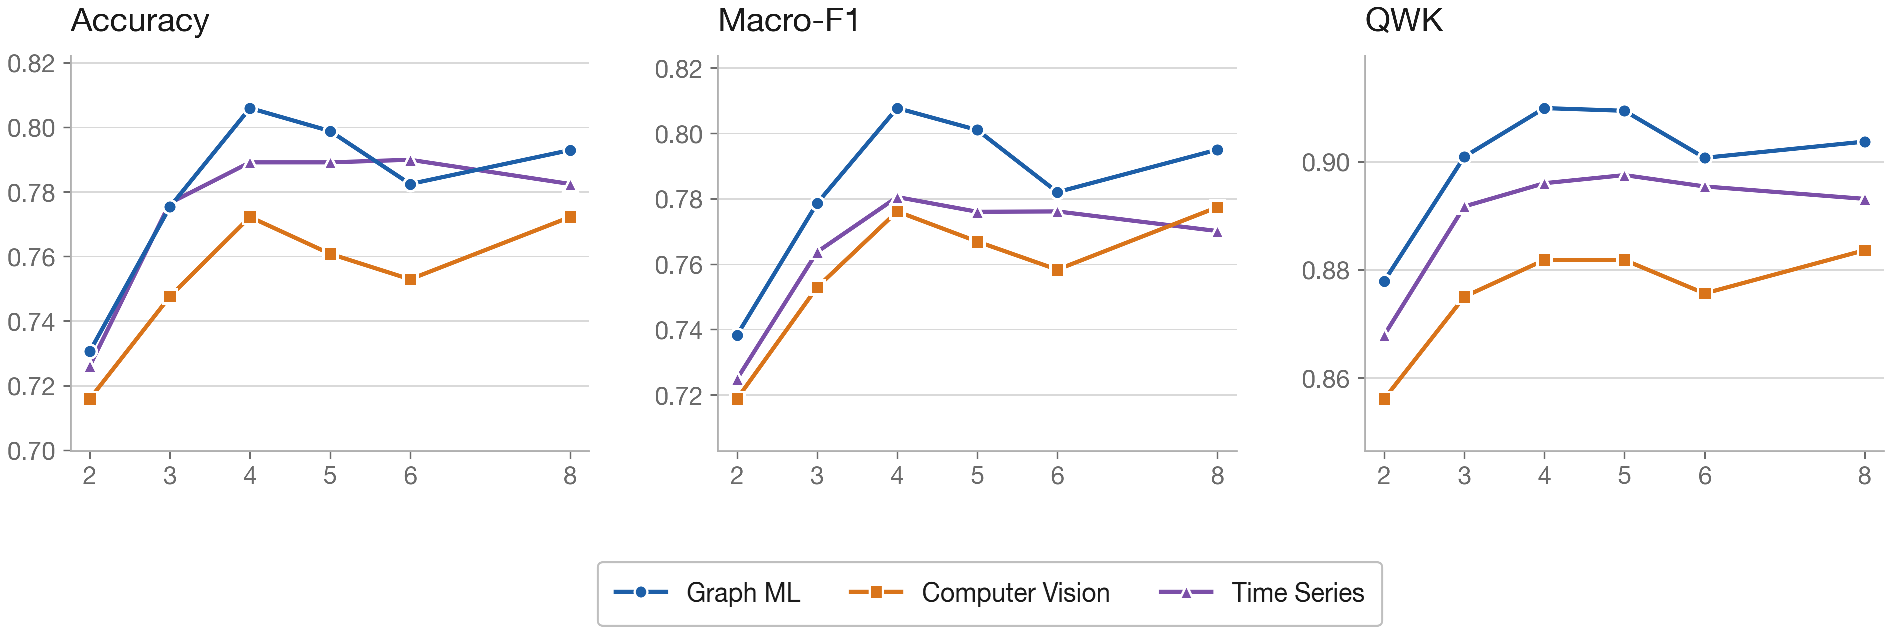
\includegraphics[width=\textwidth]{pic/param_sensitivity/topk.png}
\caption{Sensitivity to the evidence budget $K$ in the three domains. The
default is $K{=}5$, the checkpoint of Table~\ref{tab:panel-a}. $K$ is a padding
dimension, so the text reads the curves against the priors each setting
consumes.}
\label{fig:topk}
\end{figure}

\paragraph{Evidence budget: the ideas run out of priors before the model runs
out of capacity.}
Figure~\ref{fig:topk} varies $K$, the number of priors each idea contributes,
over $K=2,3,4,5,6,8$. Accuracy rises steeply from $K{=}2$ to $K{=}4$ ($0.731 \to
0.806$ on Graph ML, $0.716 \to 0.772$ on computer vision, $0.726 \to 0.789$ on
time series) and then flattens, with the same knee in all three domains. The
flattening comes from the evidence rather than from the model. Because every
sample is padded to exactly $K$ slots, the priors a setting consumes stop
growing once $K$ exceeds the candidates an idea carries, and the knee sits at
three to four consumed priors. Raising $K$ from 5 to 8 adds less than one
consumed prior, because about a third of the ideas carry six or more candidates
and fewer than one in seven carry eight or more.

\begin{figure}[h]
\centering
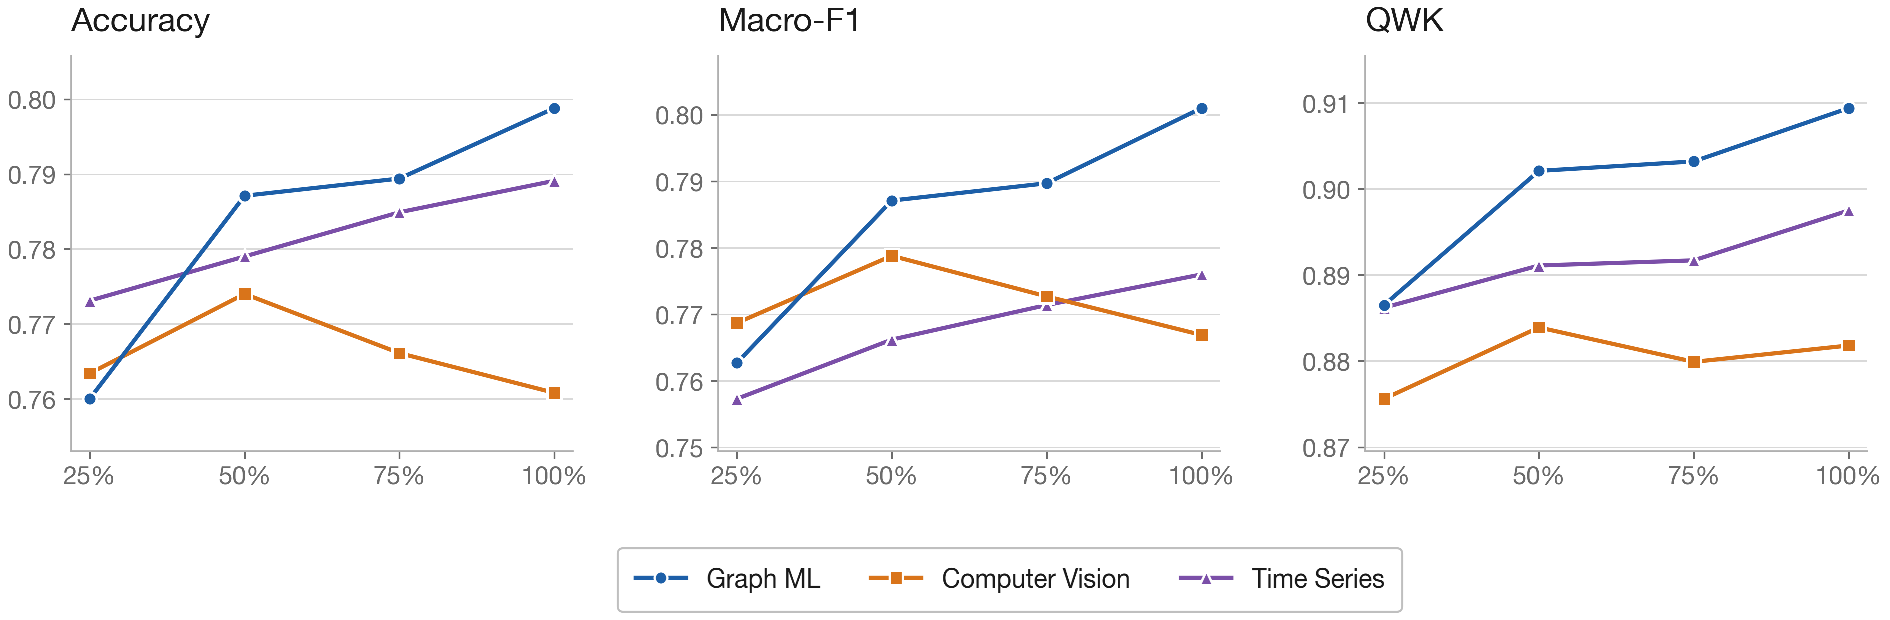
\includegraphics[width=\textwidth]{pic/param_sensitivity/train_frac.png}
\caption{Sensitivity to the amount of EGRD training data in the three domains.
Development and test sets stay fixed, and $100\%$ is the default.}
\label{fig:train-frac}
\end{figure}

\paragraph{Training-set size: more data helps across the board.}
Figure~\ref{fig:train-frac} varies the number of training ideas over $25\%$,
$50\%$, $75\%$ and $100\%$ of the training split, drawn as nested stratified prefixes so that
consecutive points add samples without reordering what came before. Macro-F1
rises steadily with the fraction on Graph ML ($0.7627 \to 0.8010$) and time
series ($0.7573 \to 0.7760$). Computer vision levels off after $50\%$ and ends
at $0.7669$ against a peak of $0.7788$, a gap of $0.012$. More training data
helps in most of the domains we measure, and the spread across the four
fractions stays small: accuracy moves by at most $0.039$ in any domain.

\begin{figure}[h]
\centering
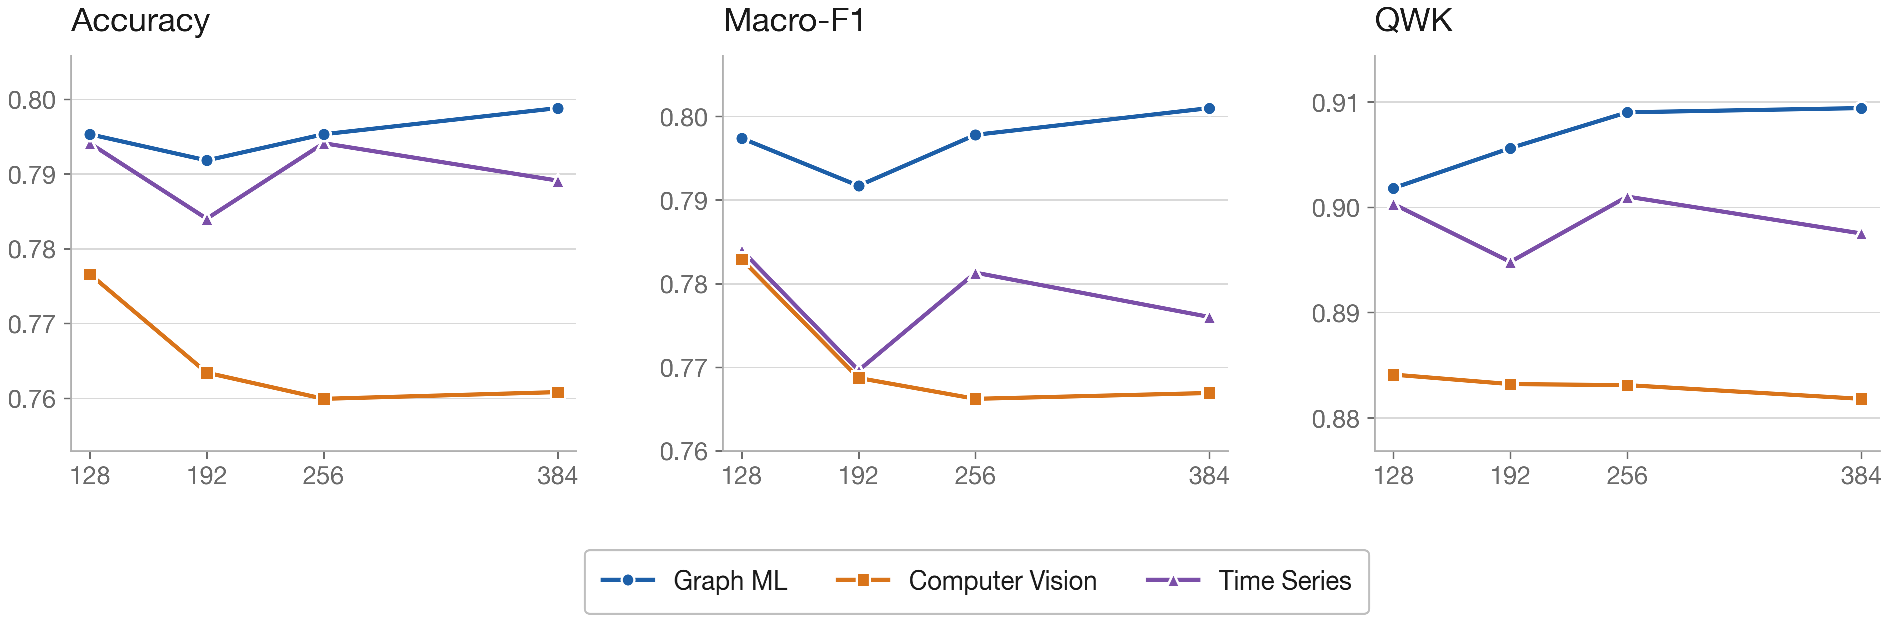
\includegraphics[width=\textwidth]{pic/param_sensitivity/max_length.png}
\caption{Sensitivity to encoder input length on the three domain test splits.
The default is 384, and every setting scores the same test ideas and labels.}
\label{fig:maxlen}
\end{figure}

\paragraph{Encoder input length: 128 tokens already cover the comparison.}
Figure~\ref{fig:maxlen} varies the encoder input length over 128, 192, 256 and
384 tokens. The four lengths separate the domains by little: no domain moves monotonically
with input length, and tripling the input moves Macro-F1 by at most $0.017$ in
any domain. At 128 tokens the encoder already covers the title-and-abstract
comparison for most target--prior pairs, so a longer window reads much the same
text and the curves stay flat. QWK is the flattest panel, spanning $0.0076$ on
Graph ML, $0.0023$ on computer vision and $0.0062$ on time series across the
four lengths, so the ordering the model produces is close to invariant to how
much of the text it reads. The flatness is consistent with the decomposition
reading a target and its priors through short unit-level comparisons rather than
through long spans of text.

\begin{table}[h]
\centering
\footnotesize
\setlength{\tabcolsep}{6pt}
\renewcommand{\arraystretch}{1.05}
\caption{Per-domain seed variability. Entries are sample standard deviations
across seeds 173, 174 and 175 with identical data, code and configuration.}
\label{tab:seed-noise}
\begin{tabular}{@{}l rrrrr@{}}
\toprule
Domain & Acc & Ma-F1 & QWK & MAE & High-F1 \\
\midrule
Graph ML & 0.0066 & 0.0050 & 0.0048 & 0.0067 & 0.0022 \\
Computer vision & 0.0040 & 0.0021 & 0.0032 & 0.0027 & 0.0037 \\
Time series & 0.0050 & 0.0045 & 0.0031 & 0.0051 & 0.0069 \\
\bottomrule
\end{tabular}
\end{table}

\paragraph{Seed stability: the reported model is not a selected seed.}
Table~\ref{tab:seed-noise} varies nothing but the random seed, running the
default configuration on seeds 173, 174 and 175 with identical data and code and
reporting the per-domain sample standard deviations. The spread is $0.004$--$0.007$ in accuracy and $0.002$--$0.005$ in Macro-F1, so
the headline numbers describe the configuration rather than one fortunate run,
and the three sweeps above should be read by the shape of a curve rather than by
the difference between adjacent points.

\section{Limitations}
\label{app:limitations}

Two bounds on the claims of this paper are worth stating directly.

\paragraph{Three domains.}
\textsc{IdeaDelta} is drawn from graph machine learning, computer vision and
time series, and the RINoBench transfer indicates what lies outside them:
roughly $30$ of its $277$ test ideas fall in these three fields, and the model
reads the remainder without ever having been trained on their literature.
Coverage of a field is what the decomposition needs, since a prior can only
support a unit of a target the model is equipped to read, so we do not claim
the reported accuracy outside the three.

\paragraph{Transfer to expert judgment is partial.}
On RINoBench the frozen checkpoint leads every baseline on the rank-sensitive
metrics, at $0.2245$ QWK and $0.3407$ Macro-F1 against $0.1469$ and $0.2457$ for
the best other system on each, and it is the only system above $0.15$ kappa. But
$0.2245$ is a modest level of agreement, and accuracy adds nothing to it: our
row reaches $0.4152$, exactly the constant predictor, with a prediction that is
not constant. What transfers is the ordering of ideas, not the grade an idea
receives. Two properties of the setting bound how far that can be pushed within
the present design: most RINoBench ideas lie outside the three fields above, and
folding the expert 1--5 scale to four levels merges a distinction the experts
chose to draw, placing $41.5\%$ of the ideas in one class. We read the result as
partial agreement with expert judgment rather than as evidence that the two
scales coincide.


\section{AI Use Statement}
\label{app:ai-use}
We used generative AI tools to assist with the construction of
\textsc{IdeaDelta}, including extracting and filtering research ideas,
assessing target--prior coverage, and annotating research novelty, as
described in Section~\ref{sec:dataset} and Appendix~\ref{app:dataset-details}.
The resulting labels are model-generated, and we manually inspected samples
from each stage of the construction pipeline. We also used generative AI tools
to polish the language of the manuscript and improve its clarity and
readability. The authors take responsibility for the final content of this
work, including its text, claims, and AI-assisted artifacts.

\section{Ethics Statement}
\label{app:ethics}
This work studies research novelty relative to a retrieved set of prior works.
The labels in \textsc{IdeaDelta} are model-generated assessments rather than
authoritative judgments of scientific merit. Incomplete retrieval, errors in
idea extraction, and biases of the annotation model may affect these
assessments, and uneven coverage across research fields may lead to unequal
reliability. The resulting scores should therefore support human examination
of the underlying evidence and should not serve as the sole basis for
publication decisions, evaluations of researchers, or allegations of
plagiarism. The synthetic priors used in the controlled validation experiment
are explicitly marked, do not represent real publications, and are excluded
from the released dataset, as described in Appendix~\ref{app:dataset-validity}.

\section{Reproducibility Statement}
\label{app:reproducibility}
Model and training code for all three stages is available for review in an
anonymized repository at
\url{https://anonymous.4open.science/r/EGRD_model-44A5}, including the
pair-coverage and joint-coverage models of Stage A, the residual decomposition
of Stage B, the novelty prediction heads of Stage C, and a single entry point
that reproduces the reported training pipeline under the hyperparameters used
in our experiments. The repository contains model and training code only; it
carries no data, checkpoints, or evaluation outputs. The construction
of \textsc{IdeaDelta}, including the
temporal admissibility rule and the annotation protocol, is described in
Section~\ref{sec:dataset} and Appendix~\ref{app:dataset-details}; the
architecture and training details are given in Appendix~\ref{app:method} and
Appendix~\ref{app:experiments}.

\end{document}
